%% LyX 2.3.7 created this file.  For more info, see http://www.lyx.org/.
%% Do not edit unless you really know what you are doing.
\documentclass[english]{article}
\usepackage[T1]{fontenc}
\usepackage[latin9]{inputenc}
\usepackage{float}
\usepackage{url}
\usepackage{amstext}
\usepackage{graphicx}

\makeatletter

%%%%%%%%%%%%%%%%%%%%%%%%%%%%%% LyX specific LaTeX commands.
%% Because html converters don't know tabularnewline
\providecommand{\tabularnewline}{\\}

%%%%%%%%%%%%%%%%%%%%%%%%%%%%%% Textclass specific LaTeX commands.
\newenvironment{lyxcode}
	{\par\begin{list}{}{
		\setlength{\rightmargin}{\leftmargin}
		\setlength{\listparindent}{0pt}% needed for AMS classes
		\raggedright
		\setlength{\itemsep}{0pt}
		\setlength{\parsep}{0pt}
		\normalfont\ttfamily}%
	 \item[]}
	{\end{list}}

\makeatother

\usepackage{babel}
\begin{document}
\title{Application of feature construction techniques in forest fire duration
prediction data}
\author{Constantina Kopitsa$^{1}$, Ioannis G. Tsoulos$^{2}$\thanks{Corresponding author. Email: itsoulos@uoi.gr},
Andreas Miltiadous$^{3}$, Vasileios Charilogis$^{4}$}
\date{$^{1}$\quad{}Department of Informatics and Telecommunications, University
of Ioannina, Greece;k.kopitsa@uoi.gr\linebreak{}
$^{2}$\quad{}Department of Informatics and Telecommunications, University
of Ioannina, Greece; itsoulos@uoi.gr\\
$^{3}\quad$Department of Informatics and Telecommunications, University
of Ioannina, Greece; a.miltiadous@uoi.gr\emph{}\\
$^{4}\quad$Department of Informatics and Telecommunications, University
of Ioannina, Greece; v.charilog@uoi.gr}
\maketitle
\begin{abstract}
From early times, humanity has expressed a profound need to predict
the future. In Ancient Greece, oracles held a place of high respect
and influence. In modern times, the quest for accurate forecasting
has shifted to the realms of research and science, empowered by advanced
computational tools, provided by Artificial Intelligence, particularly
Machine Learning. One of the fields where Machine Learning has established
fertile ground is in the domain of forest fire management. Forest
fires pose a major threat to both human and animal life, with significant
economic and social impacts. A reliable prediction system is crucial
for mitigating these effects, especially during summer months, dry
seasons, and in high-risk areas, such as the Mediterranean. This study,
explores feature construction, and selection methods, applied to forest
fire data, collected over 10 years in Greece, incorporating prevailing
weather conditions at ignition, and during suppression. By applying
techniques like Principal Component Analysis (PCA), Minimum Redundancy
Maximum Relevance (MRMR) feature selection, and Grammatical Evolution
for feature construction, this research aims to identify key factors
influencing fire duration. These techniques have become invaluable
allies in addressing complex predictive challenges, and advancing
our understanding of future events. Our approach, leverages advanced
computational methods, to analyze complex datasets, providing a deeper
understanding of the primary drivers of wildfire behavior, and enabling
more effective mitigation strategies.
\end{abstract}

\section{Introduction}

Fire has always had a dual nature, in human history. On one hand,
it has had the power to destroy civilizations, while on the other,
it has significantly contributed to the evolution, of human society.
From its destructive potential in warfare, and natural disasters,
to its transformative role in technological, and cultural advancement,
fire has shaped both, the rise, and fall of human civilizations. The
ability to harness fire for cooking, metallurgy, and warmth played
a crucial role in the development, of early human societies \cite{fire1},
while its unchecked force, has also led to widespread devastation.
This duality, underscores fire\textquoteright s paradoxical role,
in human progress: a force capable of both creation and destruction.

This notion is also evident in ancient Greek mythology, particularly
in the tale of Prometheus, who defied the gods by stealing fire, and
gifting it to humanity. This act symbolizes the transfer of divine
knowledge and power to humans, enabling progress and civilization.
The myth, underscores fire's dual role as a tool for human advancement
and as a source of conflict illustrating the tension between progress
and its ethical implications as well as the costs of rebellion and
innovation \cite{fire2}. On this matter, fire has played a multifaceted
role in human history, both through myths and through its tangible
impacts. 

Nevertheless, in the modern era, wildfires are ranked among the most
significant natural hazards \cite{fire3} with immense effects on
Earth's ecosystems, and human societies. Beyond that according the
Chair of ISO/TC 92 fire safety Mr. P. Van Hees: \textquoteleft \emph{With
losses caused by fire estimated at 1\% of the global GDP each year,
fire safety must be viewed in the broader perspective of risk management
and disaster mitigation}\textquoteright{} \cite{fire4}. 

In Figure \ref{fig:fireEconomic} it is illustrated, through a graphical
representation the economic burden from forest fires on the annual
GDP. 

\begin{figure}[H]
\begin{centering}
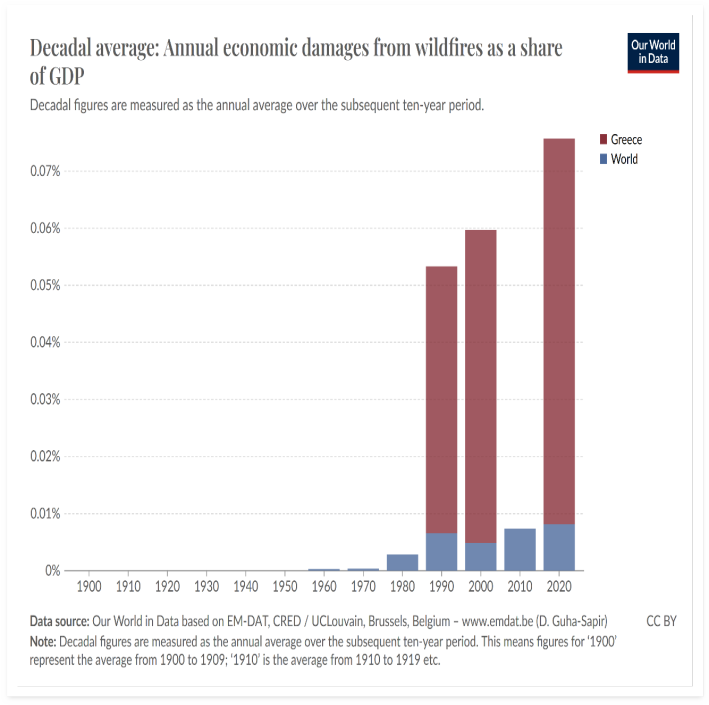
\includegraphics[scale=0.5]{fire_economic}
\par\end{centering}
\caption{The economic impact of forest fires in Greece, and around the world.\label{fig:fireEconomic}}
\end{figure}
The following numbers show the extent of the destruction caused by
fires:
\begin{itemize}
\item The cost of fire is estimated at about 1\% to 2\% of the annual GDP 
\item About 1\% of fires are responsible for more than 50\% of the costs 
\item The number of people dying in fire is estimated at 2.2 deaths per
100,000 inhabitants (based on 35 countries)\cite{fire4}. 
\end{itemize}
In other words wildfires and climate change intensify each other.
Climate change exacerbates wildfires by increasing drought, high temperatures,
low humidity, lightning, and strong winds, leading to more severe,
and prolonged fire seasons. Conversely, wildfires contribute to worsening
climate change \cite{fire5}. Thus, wildfires (along with the extraction
and burning of fossil fuels, and volcanic eruptions) exacerbate Climate
Change, by further releasing carbon dioxide, into the atmosphere \cite{fire_nasa}.
Also, the Mediterranean region is recognized as a key \textquotedbl hot-spot\textquotedbl{}
for the impacts of climate change \cite{fire_giorgi}. At the same
time, the critical need to address climate changes, effects on wildfire
patterns is highlighted as essential for protecting both the environment,
and public health in Greece \cite{fire_iliopoulos}.

In Figure \ref{fig:fireAtmosphere}, we observe the continuous increase
in carbon dioxide levels, beginning in 1751.

\begin{figure}[H]
\begin{centering}
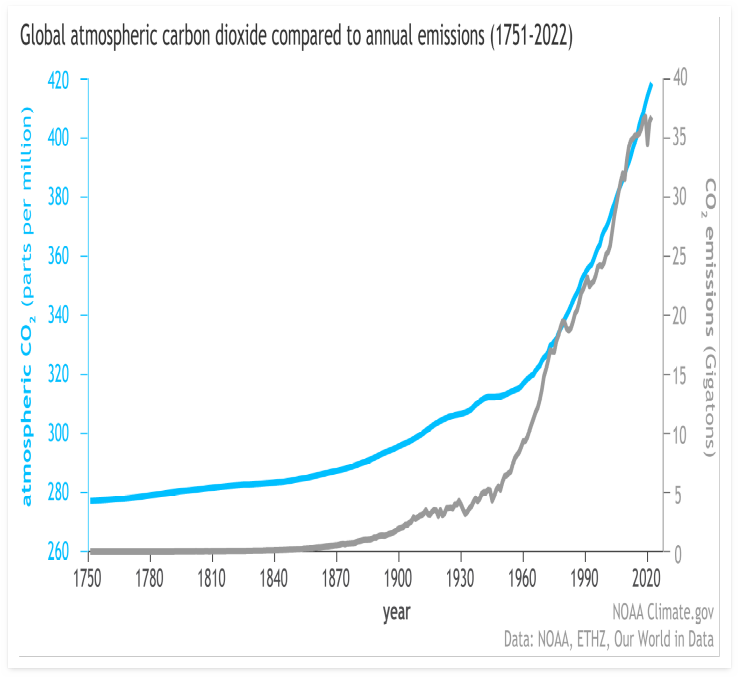
\includegraphics[scale=0.5]{fire_atmosphere}
\par\end{centering}
\caption{The environmental impact of carbon dioxide. Available from: https://www.climate.gov/news-features/understanding-climate/climate-change-atmospheric-carbon-dioxide
(accessed on November 29, 2024). \label{fig:fireAtmosphere}}
\end{figure}
Concerning this, the United Nations of Environment Programme, are
calling the governments: \textquotedblleft to radically shift their
investments in wildfires to focus on prevention and preparedness\textquotedblright{}
\cite{fire5}. Therefore, despite the challenging circumstances posed
by Climate Change, driven by continuous human expansion and technological
progress we aim to transform this disadvantage into an advantage by
focusing our efforts on advancing technology itself. On this Artificial
intelligence, particularly Machine learning, emerges as a valuable
ally in addressing this global issue, offering innovative solutions
and supporting sustainable development \cite{ai_climate,ai_ml}. 

Machine learning, refers to a collection of techniques and algorithms
that enable systems to identify patterns and make decisions based
on data improving their performance over time without explicitly being
programmed for specific tasks \cite{iso_ml}. This was the vision,
of Alan Turing, when, in 1936 he wrote his PhD \textquoteleft On Computable
Numbers, with an application to the Entscheidung problem\textquoteright{}
\cite{ml_turing}. Namely, Machine learning, is a pivotal branch of
artificial intelligence, presents endless opportunities for businesses
and society alike. Beyond its numerous advantages it plays a critical
role in driving groundbreaking advancements in Climate Change adaptation
and mitigation. By accelerating, the development of solutions, to
some of the most pressing challenges facing the planet, machine learning
is reshaping the way we address global environmental issues \cite{iso_ml}.
Although, modeling complex environmental variables, often presents
challenges due to the significant computational resources required
and the diversity or complexity of data formats \cite{ml_review}.
Machine learning algorithms, however, can bypass these challenges
by deriving mappings and relationships directly from the data eliminating
the need for predefined expert rules. This capability is particularly
beneficial when dealing with scenarios involving a large number of
parameters with intricate physical properties, such as in forest fires.
Consequently, adopting a machine learning approach to fire management
can help overcome many of the limitations associated with traditional
physics-based simulation models.

Regarding this, in the recent literature, significant interest has
been developed, in the role of machine learning in the field of fire
management \cite{fire_manage}. Forest fires, however, have not been
extensively studied as research on forest fires constitutes only 2.9\%
of the global literature, according to a study conducted between 2017
and 2021 \cite{fire_manage2}. More specifically, floods have received
the most attention in research (20.3\%), followed by earthquakes and
hurricanes, each accounting for 18.8\%. Studies on general disaster
types make up 15.9\%, while landslides account for 10.1\%. Notably,
depending on the area of focus, researchers employ corresponding algorithms
to address specific challenges.

\begin{figure}[H]
\begin{centering}
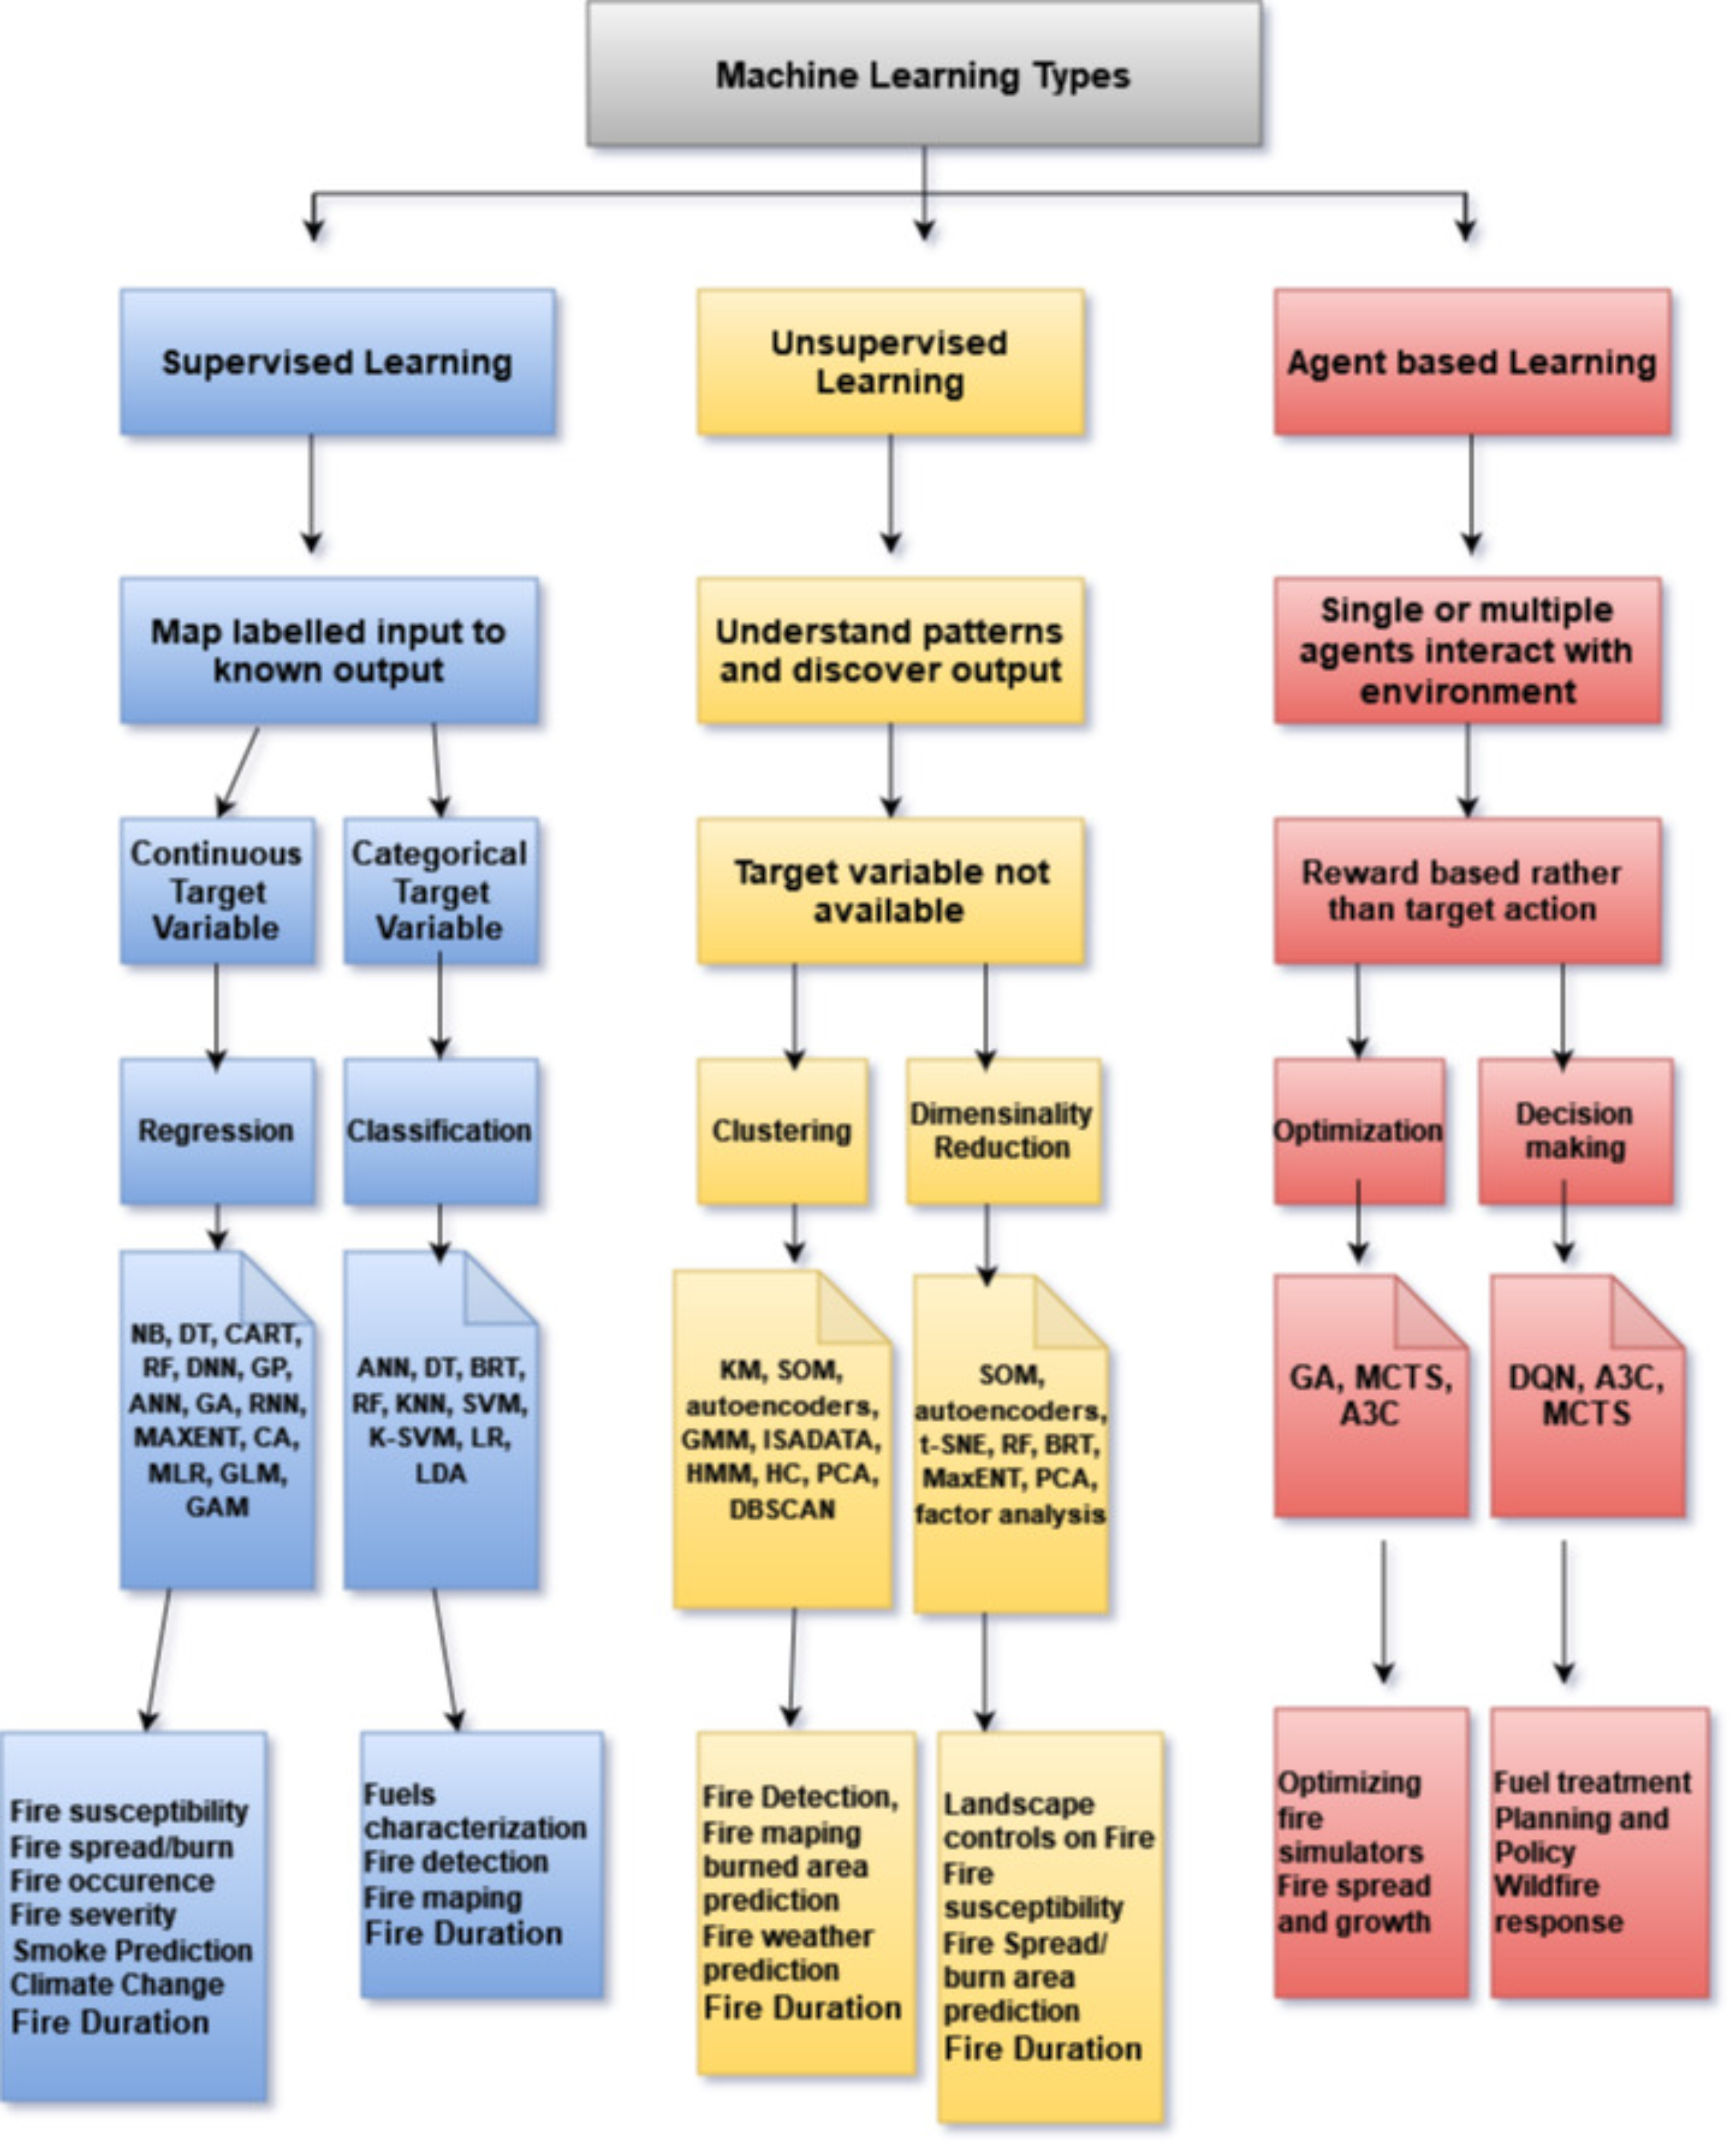
\includegraphics[scale=0.5]{fire_algorithms}
\par\end{centering}
\caption{Machine learning methods used in fire management.\label{fig:mlMethods}}
\end{figure}
Figure \ref{fig:mlMethods} summarizes the machine learning methods
used in various fields of fire management, as obtained from the relevant
literature. A number of recent publications have appeared in recent
years, which utilize machine learning techniques for forest fire management.
For example, Bayesian networks have been widely utilized in the context
of forest fires, particularly for predicting, and analyzing, potential
causes of fires \cite{fire_bayes1}. Additionally, a recent study
employed Bayesian networks to model the cascading effects of drought
and forest fires \cite{fire_bayes2}. Also, Bayesian networks were
integrated with deep learning techniques to detect fires, from video
frames \cite{fire_bayes3}.

Na�ve Bayes, has been also applied to forest fire-related challenges
in numerous studies. For instance, Nugroho developed a forest fire
prevention system, that combines a wireless sensor network with a
Na�ve Bayes classifier \cite{fire_naive1}. Zainul's work proposes
a method for classifying hotspots responsible for forest fires using
the na�ve Bayes algorithm \cite{fire_naive2}. Karo, proposed a methodology
for wildfire classification, that incorporates feature selection and
employs Na�ve Bayes alongside other machine learning techniques \cite{fire_naive3}.

Moreover, Logistic Regression, has been applied to various forest
fire-related issues, including estimating human-caused wildfire risk
\cite{fire_log1}, predicting wildfire vulnerability \cite{fire_log2},
probabilistic modeling of wildfire occurrence \cite{fire_log3} and
analyzing wildfire danger \cite{fire_log4}. 

Several studies, have utilized Artificial Neural Networks (ANNs),
in the field of forest fire prediction, and monitoring. For instance,
Hossain, employed ANNs to detect flames and smoke based on static
image features \cite{fire_ann1}. Lall and Mathibela applied neural
networks to predict wildfire risk in Cape Town \cite{fire_ann2}.
Similarly, Sayad utilized neural networks along with other machine
learning techniques for wildfire predictive modeling, using data from
NASA\textquoteright s Land Processes Distributed Active Archive Center
(LP DAAC) \cite{fire_ann3}. Additionally, Gao recently published
a case study, on predicting wildfires, in a Chinese province, using
neural networks \cite{fire_ann4}. 

Also, Random Forest, has been widely utilized in forest fire prediction.
For instance, Latifah applied Random Forest, to predict forest fires
in Borneo \cite{fire_rf1}. Similarly, Malik proposed the usage of
Random Forest to estimate the wildfire risk in Northern California
\cite{fire_rf2}. Additionally, Gao conducted a forest fire risk prediction
study in China, combining Random Forest with a neural network trained
using the back-propagation method \cite{fire_rf3}.

This paper addresses a key issue in forest fire management, such as
predicting the duration of fires, utilizing information from already
caused forest fires in combination with the weather conditions that
prevailed during the development of this phenomenon. Regarding this
topic a series of research papers have been published during the past
years, such as the work of Xiao et al \cite{fire_manage}, who developed
a wildfire duration prediction model, based on historical fire data
and geospatial information. The algorithms employed included: RF (Random
Forest), KNN, and XGBoost regression models as well as image-based
approaches such as CNN and Encoder. The model, achieved an accuracy
exceeding 80\% for fires lasting longer than 10 days. In the same
direction of research, Andela validated the fire data from the Global
Fire Atlas, using independent datasets from the United States. The
study utilized satellite data and highlighted that the duration of
fires is significantly influenced among others by the fire season
\cite{duration_andela}. Ujjwal settled a surrogate model to capture
the dynamic spread of a wildfire over time. The surrogate model, designed
to simulate the relationship between the burned area and key meteorological
parameters (such as relative humidity, temperature, and wind speed),
provides valuable insights, into fire behavior across different \cite{duration_surrogate}.
Wang, also conducted research that while capable of yielding results
for predicting, wildfire duration, primarily, focused on forecasting
the scale of a forest fire. The study utilized neural network algorithms,
including Backpropagation Neural Network (BPNN), Recurrent Neural
Network (RNN) and Long Short-Term Memory (LSTM). Among these classification
methods, LSTM demonstrated the highest accuracy, achieving 90.9\%
\cite{duration_wang}. Xi settled a framework, for jointly, modeling
fire duration, and size using a bivariate finite mixture model. Four
subpopulations (normal or extreme in duration and size) were analyzed,
incorporating, variables such as: location, month, and environmental
factors. The analysis, revealed a strong correlation between: duration,
and size, and identified key predictors, influencing these subpopulations
\cite{duration_xi}.

Predicting, the duration of a fire is crucial, as it allows for estimating
the potential damage, to the affected area and determining the necessary
human resources, for its suppression. Besides that, forest fires and
climate change are commonly exacerbating. The Western fire chief\textquoteright s
association, from the U.S. emphasizes that climate change is drastically
impacting the fire season. As a result, fire seasons now last six
to eight months, compared to the four months, they previously spanned
. Face the Facts USA reports that in the U.S. the average duration
of wildfires increased from 8 days, before 1986, to 37 days by 2013
\cite{duration_wfca}.

The current work utilizes a series of feature construction and selection
methods in order to improve the ability of various machine learning
techniques to predict the duration of forest fires. These methods
involve creating new, meaningful variables by combining or transforming
existing data attributes \cite{genfc1}. For example, integrating
material resources deployed during a forest fire event into a single
metric constitutes feature construction, enabling models, to better
capture the complexity, of fire incidents, and resource allocation.
Another example, for Feature Construction, during a forest fire, is
combining weather attributes, in order to form, a fire risk index.
Such, approaches enhance data representation, facilitating more robust,
and interpretable predictive models, in disaster management. The feature
construction or selection methods were applied on data collected for
the Greek case that contained weather information.

The remaining of this manuscript is divided as follows: section \ref{sec:Materials-and-Methods}
described the used dataset and it provided a detail discussion on
the used methods, section \ref{sec:Results} outlines the conducted
experiments and some statistical tests on them and finally section
\ref{sec:Conclusions} discusses some conclusions on the experimental
results.

\section{Materials and Methods\label{sec:Materials-and-Methods}}

This section initiates with a description of the used datasets and
continues with a detailed description of the used feature construction
and selection techniques, that will be applied on the datasets incorporated
in the conducted experiments.

\subsection{The used dataset }

In this research, open data provided by the Hellenic Fire Service
were utilized, available at the link \url{https://www.fireservice.gr/en_US/synola-dedomenon}.
The datasets used included information on all fires that occurred
in Greece during the years 2014--2021. The data encompassed the location
of the fire, the date and time of ignition and extinguishment, the
burned areas categorized by land type, and the firefighting forces
deployed for suppression efforts. 

The datasets comply with the European transparency legislation (Directive
2013/37/EU), ensuring that the data are unbiased in terms of type
and location, and represent all fires in the Hellenic region. The
information provided by the Hellenic Fire Service is easily accessible,
regularly updated, accurate, and comprehensive, facilitating analysis
and covering all involved entities. 

Regarding burned areas, the dataset included measurements for the
following categories: forests, forested areas, groves, grasslands,
reed beds and wetlands, agricultural lands, crop residues, and landfills. 

As for the firefighting units deployed, the dataset included measurements
for the following resources: firefighters, ground-based teams, volunteers,
military forces, other supporting units, fire trucks, service vehicles,
tankers, machinery, CL-215 aircraft, PZL aircraft, GRU aircraft, as
well as contracted helicopters and aircraft.

\subsubsection{Data Preprocessing and Weather Feature Extraction}

The first step in data preprocessing involved removing rows with missing
values. Subsequently, using the OpenCage Geocoding API, the location
data, initially formatted as \textquotedbl Municipality, Area, Address,\textquotedbl{}
were converted into geolocation data in the form of latitude and longitude
coordinates.

Next, weather information was extracted for each fire event using
the OpenWeather API, capturing data for both the ignition and extinguishment
times. OpenWeather is a widely used service that provides detailed
weather data, including historical, real-time, and forecasted weather
information. The extracted weather features included the following:
\begin{enumerate}
\item \textbf{Temperature at 2 meters}: The air temperature near the ground
level.
\item \textbf{Relative Humidity at 2 meters}: The percentage of moisture
in the air relative to its maximum capacity.
\item \textbf{Dew Point at 2 meters}: The temperature at which air reaches
saturation and moisture condenses.
\item \textbf{Precipitation}: The amount of rainfall during the specific
time interval.
\item \textbf{Weather Code}: A classification of the general weather conditions
(e.g., clear, cloudy, rainy).
\item \textbf{Cloud Cover}: The percentage of the sky obscured by clouds.
\item \textbf{Evapotranspiration} (ET0): The potential evapotranspiration
measured using the FAO Penman-Monteith method, indicating water loss
from the surface and vegetation.
\item \textbf{Vapour Pressure Deficit} (VPD): The difference between the
amount of moisture in the air and the maximum it can hold.
\item \textbf{Wind Speed} at 10m and 100m: Wind velocity measured at heights
of 10 meters and 100 meters.
\item \textbf{Wind Direction} at 10m and 100m: The directional angle of
the wind at the respective heights.
\end{enumerate}
\begin{quote}
Additionally, daily-level weather data were included, such as:
\end{quote}
\begin{enumerate}
\item \textbf{Daylight Duratio}n: The total hours of daylight during the
day.
\item \textbf{Sunshine Duration}: The total hours of direct sunlight during
the day.
\end{enumerate}
\begin{quote}
These features were aggregated and matched with each fire record,
ensuring comprehensive weather context for both the ignition and extinguishment
phases of the fires.
\end{quote}

\subsubsection{Definition of the output variable}

To define the output variable, the duration of each forest fire was
converted from hours or other time units into minutes, ensuring greater
precision in classification. A logarithmic transformation of fire
duration in minutes was then applied to manage the wide range of values
effectively, preventing excessive influence from extreme durations.
Based on this transformation, three distinct categories were established,
serving as target values for experimental analysis. This approach
enabled the classification of forest fires according to their duration.
For the Greek forest fire data used in this study, the following classification
scheme was adopted: 
\begin{enumerate}
\item Up to 360 minutes (6 hours) is considered to be a fire, of short duration. 
\item From 361 -- 7200 minutes (6 hours -- 5 days) is a fire of medium
duration. 
\item More than 7201 minutes (5 days - and more), which is considered a
long duration fire.
\end{enumerate}

\subsection{The used feature construction and selection methods}

\subsubsection{The PCA method }

The Principal Component Analysis (PCA) technique, introduced by mathematician
Karl Pearson in 1901 \cite{pca1}, and developed by Harold Hotelling
(1933). This technique operates on the principle that when data from
a higher-dimensional space is transformed into a lower-dimensional
space, the resulting lower-dimensional representation should retain
the maximum variance of the original data. 

Notably, it is worth mentioning that the use of PCA, on larger datasets,
became practical only after the advent of electronic computers, which
made it computationally feasible, to handle datasets, beyond trivial
sizes \cite{pca_cadima}. Continuing, with the applications of PCA,
it is a widely utilized technique in exploratory data analysis, and
machine learning, particularly, in building predictive models. It
is an unsupervised learning method, designed to analyze, the relationships
among a set of variables. Often referred to as a form of general factor
analysis, it involves regression to determine a line of best fit.
The primary objective, of PCA, is to reduce the dimensionality of
a dataset, while retaining the most significant patterns, and relationships,
among the variables, all without requiring prior knowledge, of the
target variables \cite{pca_i2}. 

Next, we will briefly reference studies, that have utilized PCA, covering
different areas, such as: statistical physics, genetic improvement,
face recognition, economic \& environmental sciences, medical prediction,
e.t.c. Explicitly, the research conducted, by Park \cite{pca_park},
highlights the reasons behind the success of the PCA technique, for
lattice systems. The study's primary limitation lies in the dependency
of the proposed formula's accuracy on the dataset size. Specifically,
the results achieve full precision, only under the condition of an
infinite dataset. This constraint restricts the practical applicability,
of the method, when working with finite or limited data, a common
scenario, in real-world analyses. 

Additionally, the work of Sarma et al. \cite{pca_sarma} utilizes
PCA, in order to evaluate, morphometric traits, under a multivariate
approach. The findings suggest, that PCA could significantly enhance
the genetic improvement. Noteworthy, is the fact, that the 64.29\%,
of the total variance explained, can be considered relatively low.
This suggests, that a significant amount of unexplained information
remains, which is not captured, by the four principal components.
Moreover, Gambardella et al. used the PCA technique for monitoring
the cultivation, of cannabis, in Albania. Specifically, with PCA they
remove redundant spectral information from multiband datasets \cite{pca_parente}.
The article, by Slavkovic and Jevtic \cite{pca_electric}, presents
the implementation of a face recognition system based on the Principal
Component Analysis (PCA) algorithm. The PCA technique was utilized
by Hargreaves \cite{pca_stock}, for stock selection, specifically
to identify, a limited number of stock variables, that could effectively
aid, in determining winning stocks. 

Moreover, Xu et al. presents an interesting example of a modified
application of Principal Component Analysis (PCA), utilizing, both
linear and non-linear methods, through Kernel PCA (KPCA), in combination,
with the Adaptive Boosting (AdaBoost) algorithm \cite{pca_kernel}.
In the study of Zhang \cite{pca_zhang}, a neural network model, combining
PCA and Levenberg-Marquardt \cite{lm_paper} was developed, to efficiently,
and accurately analyze, and predict the interaction between IAQ and
its influencing factors. In particular, it was examined indoor air
quality (IAQ), and its relationship, with building features, and environmental
conditions. 

In the work of Akinnuwesi et al \cite{pca_svm}, a hybrid approach
was suggested combining Principal Component Analysis (PCA), and Support
Vector Machine (SVM) \cite{svm}. They create, the Breast Cancer Risk
Assessment and Early Diagnosis (BC-RAED) model, designed to accurately
detect BCa, in its early stages. PCA, was initially applied to extract
features, during the first preprocessing stage, followed by further
feature reduction, in the second stage. The multi-preprocessed data,
were analyzed for breast cancer risk, and diagnosis using SVM. The
BC-RAED model, achieved, an accuracy of 97.62\%, a sensitivity of
95.24\%, and a specificity of 100\% in assessing, and diagnosing breast
cancer risk. 

Subsequently, we will briefly mention certain studies, that have been
conducted, in the field of Forest Fires. Guan's research focuses on
forest fire prediction using PCA-preprocessed data. The preprocessing
step removed irrelevant information, simplifying analysis. Linear
regression and random forest methods were then applied, revealing
temperature, relative humidity, wind, and rain as the most influential
factors in forest fire occurrence \cite{pca_guan}. 

A novel model was developed, by Nikolov, using meteorological forecast
data as input. Principal Component Analysis (PCA), with orthogonal
rotation, was applied to reduce 195 meteorological variables, from
the NARR dataset, to a smaller set of significant fire-ignition predictors,
later used in logistic regression, to calculate wildfire ignition
probabilities \cite{pca_nikolov}. Also, a recent publication focuses
on predicting wildfire ignitions, caused by lightning strikes, which
account for the largest area burned annually, in the extratropical
Northern Hemisphere. Principal Component Analysis (PCA), played a
key role, in reducing 611 potential predictors, to 13 principal components,
which were used in logistic regression to identify the primary factors
influencing lightning occurrence \cite{pca_nikolov2}. 

\subsubsection{The MRMR method }

The min-redundancy max-relevance (MRMR) algorithm, introduced by Chris
Ding and Hanchuan Peng \cite{mrmr1}. This method aims to optimize
feature selection, by minimizing redundancy, and maximizing relevance
\cite{mrmr2}. In sum, MRMR enhances relevance-only methods, such
as using an f-test between the target, and the features. When two
features are similar, MRMR prioritizes only the one, with the highest
relevance.

The study, by Zhao, extends traditional MRMR methods, by introducing
a non-linear feature redundancy measure and a model-based feature
relevance measure, which are tested on synthetic and real-world datasets.
Based on its empirical success, MRMR is integrated into Uber's marketing
machine learning platform to automate the creation and deployment
of scalable targeting and personalization models \cite{mrmr_zhao}. 

Moreover, Wu et al. proposed that the MRMR algorithm is utilized in
conjunction with a Random Forest model \cite{random_forest} to perform
feature selection in the context of air quality prediction. MRMR,
is employed to determine which variables have the most significant
impact, on the air quality index (AQI), while minimizing redundancy
among them \cite{mrmr_wu}. 

The article, by Elbeltagi is an innovative approach for estimating
maize chlorophyll by integrating hyperspectral indices with cutting-edge,
six advanced machine learning techniques. The MRMR algorithm was incorporated
into the process to enhance feature selection by pinpointing the most
significant spectral bands, minimizing data redundancy and boosting
model efficiency \cite{mrmr_elbeltagi}. 

In the energy sector, Liu conducted the following research offering
an improved method for predicting transient stability in power systems.
The MRMR algorithm is applied for feature selection with minimal redundancy
and maximum relevance providing an enhanced approach for forecasting
transient stability, in power systems. This approach addresses the
limitations of previous methods, such as low accuracy, difficult applicability
and high computational cost, while incorporating the \textquotedbl winner
take all\textquotedbl{} (WTA) technique for ensemble learning and
enhanced precision \cite{mrmr_liu}. 

Eristi also refers to the energy sector. Specifically, this paper
presents, a new PD detection system, that combines spectral analysis,
spectrogram analysis, deep learning algorithms, MRMR and ensemble
machine learning (EML) \cite{eml}. The most impactful features, are
identified, by performing MRMR feature selection analysis, on the
extracted deep features \cite{mrmr_eristi}.

Zhang employed an Acoustic Emission (AE) technique to monitor inaccessible
areas of large storage tank floors utilizing AE sensors positioned
externally to the tank. The implemented algorithm effectively distinguishes
corrosion signals from interference signals, particularly drop-back
signals induced by condensation. Experimental studies were conducted
both in laboratory settings and in field environments, focusing on
Q235 steel. Seven characteristic AE features derived from signal hits
and frequency were extracted and subsequently selected for pattern
recognition, using the MRMR method \cite{mrmr_zhang}. 

Additionally, Karamouz et al., proposed a methodology to examine the
effects of climate change on sea level variations in coastal areas
using an artificial neural network model. Feature selection techniques,
including MRMR and Mutual Information (MI) are employed to identify
the most suitable predictors for the neural network input \cite{mrmr_razmi}. 

\subsubsection{The Neural Network Construction method }

Another machine learning method introduced recently that is based
on Grammatical Evolution \cite{ge1} is the construction of artificial
neural networks \cite{nnc}. In this work the architecture of the
neural network is produced through a series of generations of the
underlying genetic algorithm by reducing the training error of the
neural network. Furthermore, the method is able to identify the best
set of parameters for the neural network. This method can also retain
only a small portion of features from the original objective problem,
significantly reducing the information required to reduce the training
error. This method was used in a series of practical problems, such
as the identification of amide I bonds \cite{nnc_amide1}, solution
of differential equations \cite{nnc_de},\textbf{ }incorporation in
the detection of Parkinson's disease \cite{nnc_feas},\textbf{ }usage
in the estimation of performance of students \cite{nnc_student},
autism screening \cite{nnc_autism} etc. 

The used grammar for the construction of neural networks expressed
in Backus--Naur (BNF) form \cite{bnf1} is shown in Figure\textbf{
}\ref{fig:nncGrammar}. Numbers in parentheses represent the sequence
number of each production rule. The constant $n$ stands for the number
of input features.\textbf{}
\begin{figure}[H]
\begin{lyxcode}
\textbf{S:=<sigexpr>~~~~~~~~~~~~~~~~~~~~~~~~~~(0)}

\textbf{<sigexpr>::=<Node>~~~~~~~~~~~~~~~~~~~~(0)}

\textbf{~~~~~~~~~~~|~<Node>~+~<sigexpr>~~~~~~~(1)}

\textbf{<Node>::=<number>{*}sig(<sum>+<number>)~(0)}

\textbf{<sum>::=~<number>{*}<xxlist>~~~~~~~~~~~~(0)}

\textbf{~~~~~~~~~~~|~~~~<sum>+<sum>~~~~~~~~~~~(1)}

\textbf{<xxlist>::=~x1~~~~~~~~(0)}

\textbf{~~~~~~~~~~~~~|~~~~x2~~(1)}

\textbf{~~~~~~~~~~~~~..............}

\textbf{~~~~~~~~~~~~~|~~~~xn~~(n-1)}

\textbf{<number>::=~(<digitlist>.<digitlist>)~~~~~~~~(0)}

\textbf{~~~~~~~~~~~~~|~~~~(-<digitlist>.<digitlist>)~(1)}

\textbf{<digitlist>::=~<digit>~~~~~~~~~~~~(0)}

\textbf{~~~~~~~~~~~~~|~<digit><digitlist>~(1)}

\textbf{<digit>::=~0~~~~~~(0)}

\textbf{~~~~~~~~~~~~~|~~1~(1)}

\textbf{~~~~~~~~~~~~~...........}

\textbf{~~~~~~~~~~~~~|~~9~(9)}
\end{lyxcode}
\textbf{\caption{The grammar incorporated in the construction of neural networks.\label{fig:nncGrammar}}
}
\end{figure}
\textbf{ }This grammar produces artificial neural networks in the
following form:

\textbf{
\begin{equation}
\text{NN}\left(\overrightarrow{x},\overrightarrow{w}\right)=\sum_{i=1}^{H}w_{(n+2)i-(n+1)}\sigma\left(\sum_{j=1}^{n}x_{j}w_{(n+2)i-(n+1)+j}+w_{(n+2)i}\right)\label{eq:nn}
\end{equation}
}The symbol $H$ defines the number of processing nodes (weights).\textbf{
}The sigmoid function $\sigma(x)$ is used as the activation function
of neural network and it is defined as: 
\begin{equation}
\sigma(x)=\frac{1}{1+\exp(-x)}\label{eq:sig}
\end{equation}
The main steps of the algorithm are:
\begin{enumerate}
\item \textbf{Initialization step}.
\begin{enumerate}
\item \textbf{Set} the number of used chromosomes $N_{c}$. Each chromosome
is a set of randomly selected integers. These integer values represent
rule number in the extended BNF grammar previously presented.
\item \textbf{Set} the maximum number of allowed generations $N_{g}$.
\item \textbf{Set} the selection rate $p_{s}\in[0,1]$ and the mutation
rate $p_{m}\in[0,1]$.
\item \textbf{Set} $k=0$, the generation number.
\end{enumerate}
\item \textbf{Fitness calculation step}.
\begin{enumerate}
\item \textbf{For} each chromosome $g_{i},\ $$i=1,\ldots,N_{c}$ \textbf{do}
\begin{enumerate}
\item \textbf{Create} using the grammar of figure \ref{fig:nncGrammar}
the corresponding neural network $\mbox{NN}_{i}\left(\overrightarrow{x},\overrightarrow{w}\right)$
\item \textbf{Set} as $f_{i}=\sum_{j=1}^{M}\left(\mbox{NN}_{i}\left(\overrightarrow{x}_{j},\overrightarrow{w_{i}}\right)-y_{j}\right)^{2}$
the fitness of chromosome $i$. The set $\left(\overrightarrow{x_{j}},y_{j}\right),\ j=1,...,M$
stands for the train set of the objective problem.
\end{enumerate}
\item \textbf{End For}
\end{enumerate}
\item \textbf{Genetic operations step}.
\begin{enumerate}
\item Application of Selection operator. The chromosomes of the population
are sorted according to their fitness values and the best $\left(1-p_{s}\right)\times N_{c}$
chromosomes are copied to the next generation. The remaining are replaced
by new chromosomes produced during crossover and mutation.
\item Application of Crossover operator. In this step $p_{s}\times N_{c}$
new chromosomes will be created from the original ones. For each set
$c_{1},\ c_{2}$ of new chromosomes that will be created, two chromosomes
$g_{a}$ and $g_{b}$ are selected from the old population using tournament
selection. The new chromosomes are created using one - point crossover
between $g_{a}$ and $g_{b}$. An example of this operation is shown
graphically in Figure \ref{fig:onePoint}. 
\item Application of Mutation operator. For each element of every chromosome
a random number $r\in[0,1]$ is selected. The corresponding element
is changed randomly when $r\le p_{m}$.
\end{enumerate}
\item \textbf{Termination check step}.
\begin{enumerate}
\item \textbf{Set} $k=k+1$
\item \textbf{If} $k\le N_{g}$ then goto Fitness Calculation Step.
\end{enumerate}
\item \textbf{Application to the test set}.
\begin{enumerate}
\item \textbf{Obtain} the best chromosome $g^{*}$ from the genetic population.
\item \textbf{Create} the corresponding neural network $\mbox{NN}^{*}\left(\overrightarrow{x},\overrightarrow{w}\right)$
\item \textbf{Apply} this neural network to the test set of the objective
problem and report the corresponding error (test error).
\end{enumerate}
\end{enumerate}
\begin{figure}[H]
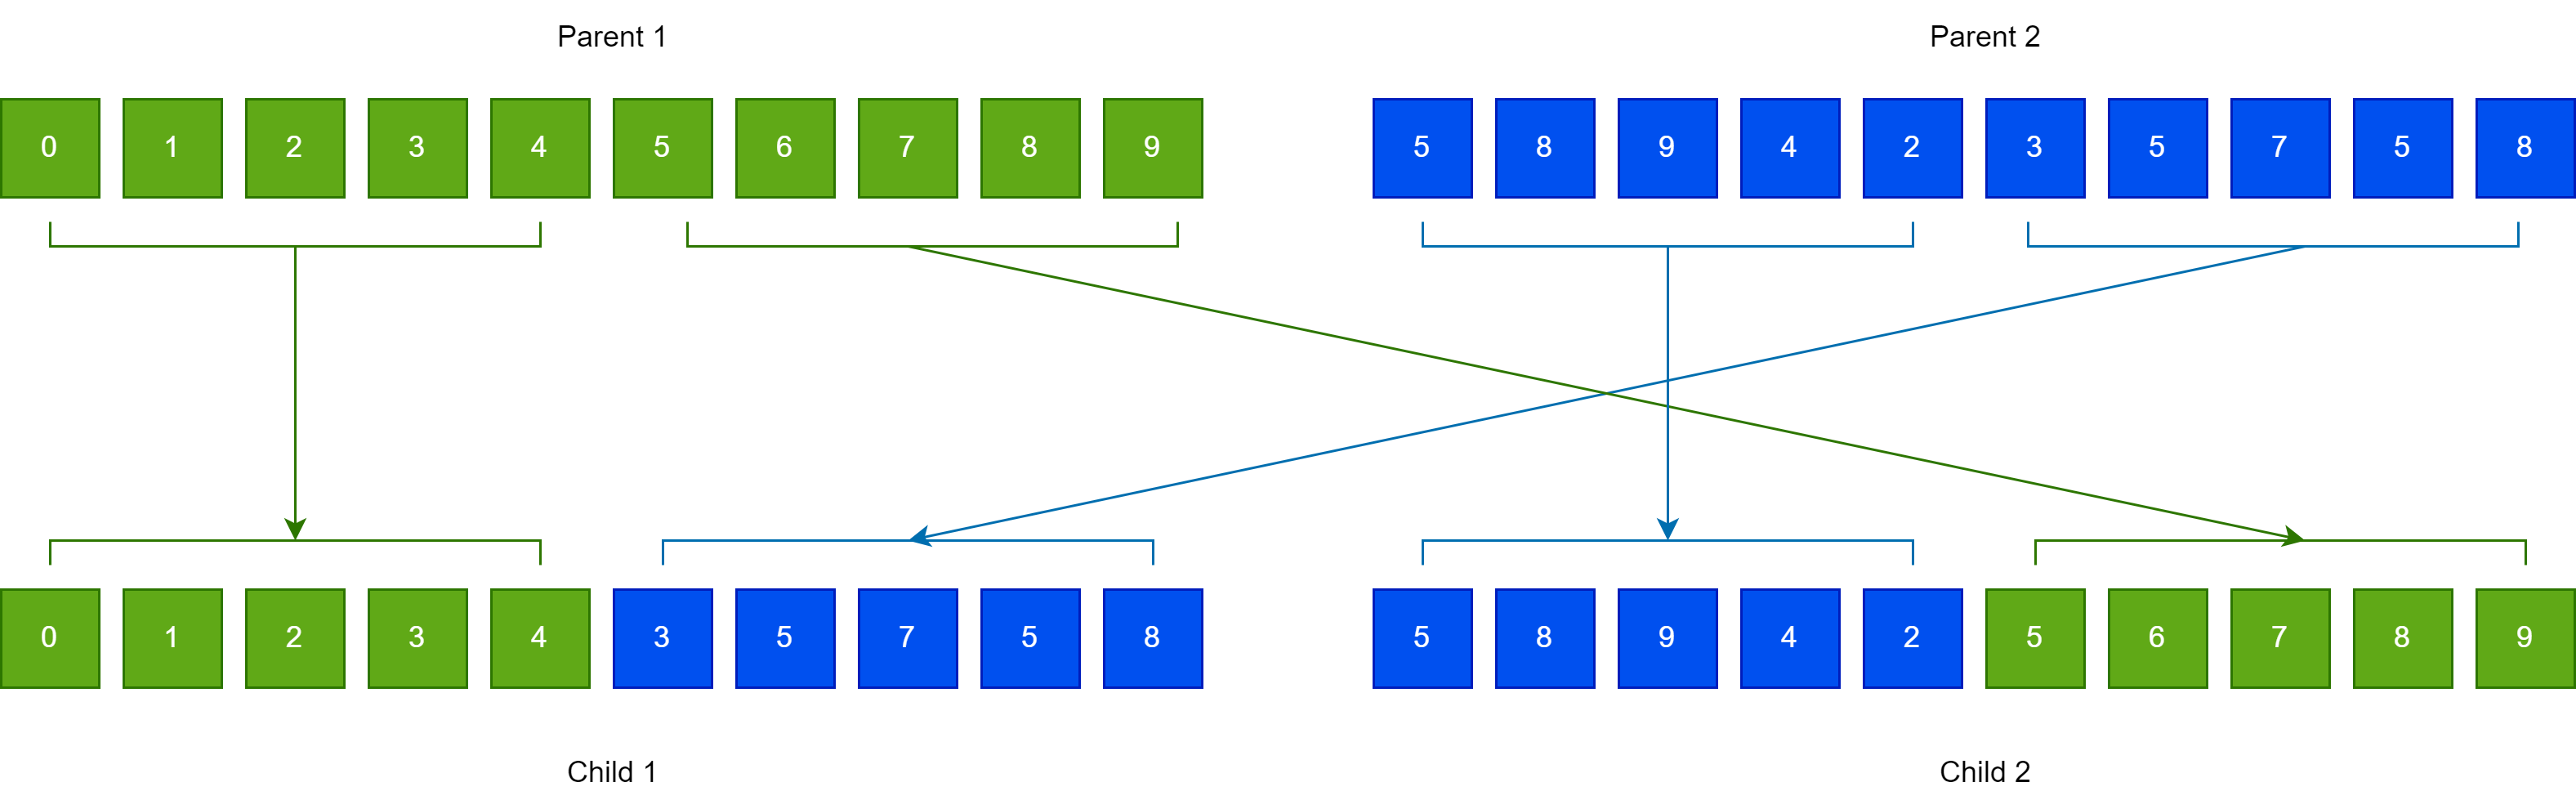
\includegraphics[scale=0.5]{onePointCrossover}

\caption{An example of the one - point crossover operation used in Grammatical
Evolution.\label{fig:onePoint}}
\end{figure}


\subsubsection{The Feature Construction method}

Another approach discussed here and used in the conducted experiments
is the feature construction technique initially proposed in \cite{fc1}.\textbf{
}This approach creates artificial features from the original ones
using the Grammatical Evolution procedure. The new features are non
- linear mappings of the original ones. This method has been used
in a series of practical cases during the past years, such as Spam
Identification \cite{fc2}, Fetal heart classification \cite{fc3},
EEG signal processing \cite{fc4,fc5} etc. The extended version of
BNF grammar used during the feature construction process is outlined
in Figure \ref{fig:fcGrammar}.

\begin{figure}[H]
\caption{The extended BNF grammar used in the feature construction process.\label{fig:fcGrammar}}

\begin{lyxcode}
S::=<expr>~~~(0)~

<expr>~::=~~(<expr>~<op>~<expr>)~~(0)~~~~~~~~~~~~~

~~~~~~~~~~~|~<func>~(~<expr>~)~~~~(1)~~~~~~~~~~~~~

~~~~~~~~~~~|<terminal>~~~~~~~~~~~~(2)~

<op>~::=~~~~~+~~~~~~(0)~~~~~~~~~~~~~

~~~~~~~~~~~|~-~~~~~~(1)~~~~~~~~~~~~~

~~~~~~~~~~~|~{*}~~~~~~(2)~~~~~~~~~~~~~

~~~~~~~~~~~|~/~~~~~~(3)

<func>~::=~~~sin~~(0)~~~~~~~~~~~~~

~~~~~~~~~~~|~cos~~(1)~~~~~~~~~~~~~

~~~~~~~~~~~|exp~~~(2)~~~~~~~~~~~~~

~~~~~~~~~~~|log~~~(3)

<terminal>::=<xlist>~~~~~~~~~~~~~~~~(0)~~~~~~~~~~~~~~~~~~~~~~

~~~~~~~~~~~|<digitlist>.<digitlist>~(1)

<xlist>::=x1~~~~(0)~~~~~~~~~~~~~~

~~~~~~~~~~~|~x2~(1)~~~~~~~~~~~~~~

~~~~~~~~~~~\dots \dots \dots{}~~~~~~~~~~~~~

~~~~~~~~~~~|~xn~(n-1)

<digitlist>::=<digit>~~~~~~~~~~~~~~~~~~(0)~~~~~~~~~~~~~~~~~

~~~~~~~~~~~|~<digit><digit>~~~~~~~~~~~~(1)

~~~~~~~~~~~|~<digit><digit><digit>~~~~~(2)

<digit>~~::=~0~(0)~~~~~~~~~~~~~

~~~~~~~~~~~|~1~(1)~~~~~~~~~~~~~

~~~~~~~~~~~.......~~~~~~~~~~

~~~~~~~~~~~|~9~(9)
\end{lyxcode}
\end{figure}
The main steps of the used algorithm have as follows:
\begin{enumerate}
\item \textbf{Initialization step}.
\begin{enumerate}
\item \textbf{Define }the number of used chromosomes $N_{c}$. 
\item \textbf{Define} the maximum number of allowed generations $N_{g}$.
\item \textbf{Set} the selection rate $p_{s}\in[0,1]$ and the mutation
rate $p_{m}\in[0,1]$.
\item \textbf{Set} as $N_{f}$ the number of desired features that will
be created.
\item \textbf{Set} $k=0$, the generation number.
\end{enumerate}
\item \textbf{Fitness calculation step}.
\item \textbf{For $i=1,\ldots,N_{c}$ do}

\begin{enumerate}
\item \textbf{Create} with the assistance of Grammatical Evolution, a set
of $N_{f}$ artificial features from the original ones, for chromosome
$g_{i}$.
\item \textbf{Transform} the original train set using the previously produced
features. Represent the new set as $\mbox{TR}=\left(x_{g_{i},j},t_{j}\right),\ j=1,..M$
\item \textbf{Apply }a machine learning model denoted as $C$ on set TR
and train this model and denote as $C(x)$ the output of this model
for any input pattern $x$.
\item \textbf{Calculate} the fitness $f_{i}$ as:
\begin{equation}
f_{i}=\sum_{j=1}^{M}\left(C\left(x_{g_{i},j}\right)-t_{j}\right)^{2}
\end{equation}
The Radial Basis Function (RBF) networks \cite{rbf1,rbf2} were used
as the machine learning models $C(x)$ in the current work. This machine
learning model was chosen because of the significantly shorter training
time it requires compared to other machine learning models. 
\end{enumerate}
\item \textbf{End For}
\item \textbf{Genetic operations step. }Perform the same genetic operators
as in the case of construction neural networks, discussed previously.
\item \textbf{Termination check step}.
\begin{enumerate}
\item \textbf{Set} $k=k+1$
\item \textbf{If} $k\le N_{g}$ then goto Fitness Calculation Step.
\end{enumerate}
\item \textbf{Application to the test set}.
\begin{enumerate}
\item \textbf{Obtain} the chromosome $g^{*}$ with the lowest fitness value.
\item \textbf{Create} the $N_{f}$ artificial features that correspond to
this chromosome
\item \textbf{Apply} the $N_{f}$ features to the train set and produce
the mapped training set $\mbox{TR}=\left(x_{g_{i},j},t_{j}\right),\ j=1,..M$
\item \textbf{Train} a machine learning model on the produced training set.
An artificial neural network \cite{nn1,nn2} with $H=10$ processing
nodes is used in the current work. This neural network was trained
using a BFGS variant of Powell \cite{powell}. 
\item \textbf{Apply} the new features to the test set of the objective problem
and create the set $\mbox{TT=}\left(x_{g_{i},j},t_{j}\right),\ j=1,..K$
\item \textbf{Apply} the machine learning model on set TT and report the
test error.
\end{enumerate}
%
\end{enumerate}

\section{Results\label{sec:Results}}

The experiments were executed using the freely available optimization
environment of Optimus, that can be downloaded from \url{https://github.com/itsoulos/GlobalOptimus.git}
as well as the WEKA programming tool \cite{weka_main}.\textbf{ }The
WEKA software has been incorporated in a series of problems \cite{weka_education1,weka_education2,weka_medical1,weka_medical2}.
Each experiment was conducted 30 times, using different seed for the
random generator each time and the ten - fold cross validation procedure
was used to validate the experimental results. The values of parameters
for the used methods are shown in Table\textbf{ }\ref{tab:expr}.\textbf{
}The following notation is used in the tables presenting the experimental
results:
\begin{enumerate}
\item The column YEAR denotes the year of recording.
\item The column BAYES the application of the Naive Bayes \cite{naive_bayes}
method to the corresponding dataset.
\item The column ADAM represents the usage of the ADAM optimizer \cite{nn_adam}
for the training of a neural network with $H=10$ processing nodes.
\item The column BFGS denotes the incorporation of the BFGS optimizer \cite{powell}
to train a neural network with $H=10$ processing nodes.
\item The column MRMR denotes the results obtained by the application of
a neural network trained with the BFGS optimizer on two features selected
using the MRMR technique.
\item The column PCA stands for the results obtained by the application
of a neural network trained with the BFGS optimizer on two features
created using the PCA technique. The PCA variant implemented in MLPACK
software \cite{mlpack} was incorporated to create these features.
\item The column NNC denotes the usage of the method of Neural Network Construction
on the proposed datasets. The software that implements this method
was obtained from \cite{nnc_softx}.
\item The column FC represents the usage of the previously mentioned method
for constructing artificial features. For the purposes of this article
two artificial features were created. These features were produced
and evaluated using the QFc software \cite{qfc}.
\end{enumerate}
\begin{table}[H]
\caption{Experimental results using a series of machine learning methods for
the prediction of forest fire duration.\label{tab:expr}}

\centering{}{\footnotesize{}}%
\begin{tabular}{|c|c|c|c|c|c|c|c|}
\hline 
{\footnotesize{}YEAR} & {\footnotesize{}BAYES} & {\footnotesize{}ADAM} & {\footnotesize{}BFGS} & {\footnotesize{}MRMR} & {\footnotesize{}PCA} & {\footnotesize{}NNC} & {\footnotesize{}FC}\tabularnewline
\hline 
\hline 
{\footnotesize{}2014} & {\footnotesize{}11.41\%} & {\footnotesize{}13.00\%} & {\footnotesize{}12.38\%} & {\footnotesize{}9.68\%} & {\footnotesize{}15.50\%} & {\footnotesize{}9.21\%} & {\footnotesize{}8.04\%}\tabularnewline
\hline 
{\footnotesize{}2015} & {\footnotesize{}10.49\%} & {\footnotesize{}11.94\%} & {\footnotesize{}11.25\%} & {\footnotesize{}8.49\%} & {\footnotesize{}15.03\%} & {\footnotesize{}9.17\%} & {\footnotesize{}7.51\%}\tabularnewline
\hline 
{\footnotesize{}2016} & {\footnotesize{}10.79\%} & {\footnotesize{}12.95\%} & {\footnotesize{}11.88\%} & {\footnotesize{}9.45\%} & {\footnotesize{}12.93\%} & {\footnotesize{}10.12\%} & {\footnotesize{}8.60\%}\tabularnewline
\hline 
{\footnotesize{}2017} & {\footnotesize{}53.36\%} & {\footnotesize{}12.68\%} & {\footnotesize{}12.65\%} & {\footnotesize{}12.65\%} & {\footnotesize{}12.64\%} & {\footnotesize{}12.61\%} & {\footnotesize{}12.66\%}\tabularnewline
\hline 
{\footnotesize{}2018} & {\footnotesize{}9.39\%} & {\footnotesize{}10.48\%} & {\footnotesize{}14.97\%} & {\footnotesize{}9.21\%} & {\footnotesize{}10.49\%} & {\footnotesize{}9.29\%} & {\footnotesize{}7.72\%}\tabularnewline
\hline 
{\footnotesize{}2019} & {\footnotesize{}7.79\%} & {\footnotesize{}9.44\%} & {\footnotesize{}9.66\%} & {\footnotesize{}8.39\%} & {\footnotesize{}9.72\%} & {\footnotesize{}7.03\%} & {\footnotesize{}6.62\%}\tabularnewline
\hline 
{\footnotesize{}2020} & {\footnotesize{}40.26\%} & {\footnotesize{}9.56\%} & {\footnotesize{}9.80\%} & {\footnotesize{}9.55\%} & {\footnotesize{}9.76\%} & {\footnotesize{}9.50\%} & {\footnotesize{}9.61\%}\tabularnewline
\hline 
{\footnotesize{}2021} & {\footnotesize{}11.81\%} & {\footnotesize{}11.06\%} & {\footnotesize{}12.90\%} & {\footnotesize{}10.57\%} & {\footnotesize{}11.03\%} & {\footnotesize{}10.80\%} & {\footnotesize{}9.55\%}\tabularnewline
\hline 
\textbf{\footnotesize{}AVERAGE} & \textbf{\footnotesize{}19.41\%} & \textbf{\footnotesize{}11.39\%} & \textbf{\footnotesize{}11.94\%} & \textbf{\footnotesize{}9.75\%} & \textbf{\footnotesize{}12.14\%} & \textbf{\footnotesize{}9.72\%} & \textbf{\footnotesize{}8.79\%}\tabularnewline
\hline 
\end{tabular}{\footnotesize\par}
\end{table}
Table \ref{tab:expr} presents the percentage values of classification
error for various machine learning models from 2014 to 2021, as well
as the average error rate for each model. The analysis reveals significant
insights regarding the performance and stability of the methods. The
BAYES model exhibits the highest variability, with a particularly
high error rate in 2017 (53.36\%). This is a clear outlier, possibly
due to specific conditions in the data or the evaluation framework.
In other years, its error rates range between 7.79\% and 11.81\%.
The average error rate for BAYES is 19.41\%, the highest in the table,
indicating the lowest overall accuracy compared to the other models.
The ADAM model shows an average error rate of 11.39\%, with values
ranging from 9.44\% to 13.00\%. Its stability is evident, as there
are no significant deviations in specific years. ADAM's performance
is considered relatively good compared to other methods. The BFGS
model has an average error rate of 11.94\%, slightly higher than ADAM's.
Its error rates range from 9.66\% to 14.97\%. Although it demonstrates
stable performance, its higher average value suggests slightly lower
accuracy in certain cases. The MRMR model has an average error rate
of 9.75\%, ranking it among the most accurate methods. However, its
error rate reaches 12.65\% in 2017, while remaining low in other years,
making it a reliable option overall. The PCA model has an average
error rate of 12.14\%, which is among the highest in the table. It
shows relatively stable values, with a slight increase to 15.50\%
in 2014. Despite its generally good performance, its accuracy is lower
compared to other methods such as MRMR or FC. The NNC model has an
average error rate of 9.72\%, one of the lowest in the table. Its
values range from 7.03\% to 12.61\%, with small deviations, demonstrating
stability and reliability. The FC model has the lowest average error
rate in the table, at 8.79\%, making it the most accurate method overall.
Its error rates range between 6.62\% and 12.66\%, indicating stable
performance with minor fluctuations. In conclusion, FC is the most
accurate model, with the lowest average error rate, while BAYES demonstrates
the lowest accuracy due to its high average error rate and significant
variability. Methods such as MRMR and NNC are also reliable, with
low error rates and relatively stable performance. The observed deviations
in specific years might be related to changes in the data or evaluation
parameters.

In Figure \ref{fig:statExper}, the results of the Wilcoxon test for
pairwise comparisons of the classification models are presented, providing
valuable insights into the statistical significance of their performance
differences. Below is a more in-depth analysis, focusing on the interpretation
of results and a deeper understanding of the relationships between
the models. The overall result of the Wilcoxon test (p < 0.5) confirms
that statistically significant differences exist among the models'
performances. This indicates that the models are not equivalent in
terms of their accuracy, with some clearly outperforming others. The
comparison between FC and NNC (p = 0.039) reveals a statistically
significant difference, though the p-value is relatively close to
the significance threshold (commonly p < 0.05). This suggests that
while FC outperforms NNC, the difference is not exceedingly pronounced.
This outcome might be influenced by specific data characteristics
or variations in the models' stability. The comparison between FC
and PCA (p = 0.016) shows a clearer statistically significant difference.
FC's performance is evidently superior to PCA\textquoteright s, which
may be attributed to the fundamental differences in their methodologies.
PCA, as a dimensionality reduction technique, might lose critical
information in the data, leading to lower accuracy in certain scenarios.
For the comparison between FC and MRMR (p = 0.039), a statistically
significant difference is observed once again. Similar to the FC-NNC
comparison, this difference exists but is not highly pronounced. MRMR,
which selects features based on mutual information, might not perform
as consistently across all datasets, giving FC an edge. The comparison
between FC and BFGS (p = 0.016) indicates an even more distinct difference.
BFGS, as an optimization method, may lack the flexibility or precision
required for classification tasks, allowing FC to demonstrate more
stable and superior performance in this case. The difference between
FC and ADAM (p = 0.023) is also statistically significant. While ADAM
is generally considered an effective algorithm in many contexts, FC
appears to outperform it in this analysis, possibly due to better
adaptability to the specific characteristics of the dataset. The most
striking difference is seen in the comparison between FC and BAYES
(p = 0.0078). The very low p-value strongly confirms a statistically
significant difference, highlighting FC\textquoteright s clear superiority
over BAYES. Notably, BAYES has exhibited high variability in its performance,
especially in 2017, when it recorded a very high error rate. This
variability likely reduces its overall reliability, which is reflected
in this comparison. In summary, FC consistently outperforms all other
models in this analysis, with statistically significant differences
observed in all pairwise comparisons. The differences are not only
numerical but also conceptual, as FC\textquoteright s superior performance
can likely be attributed to its stability, flexibility, and ability
to handle the data\textquoteright s nuances more effectively. In contrast,
models like BAYES and PCA seem more affected by changes in the data
or problem conditions. This analysis highlights FC as the most reliable
and high-performing model among those evaluated.

\begin{figure}[H]
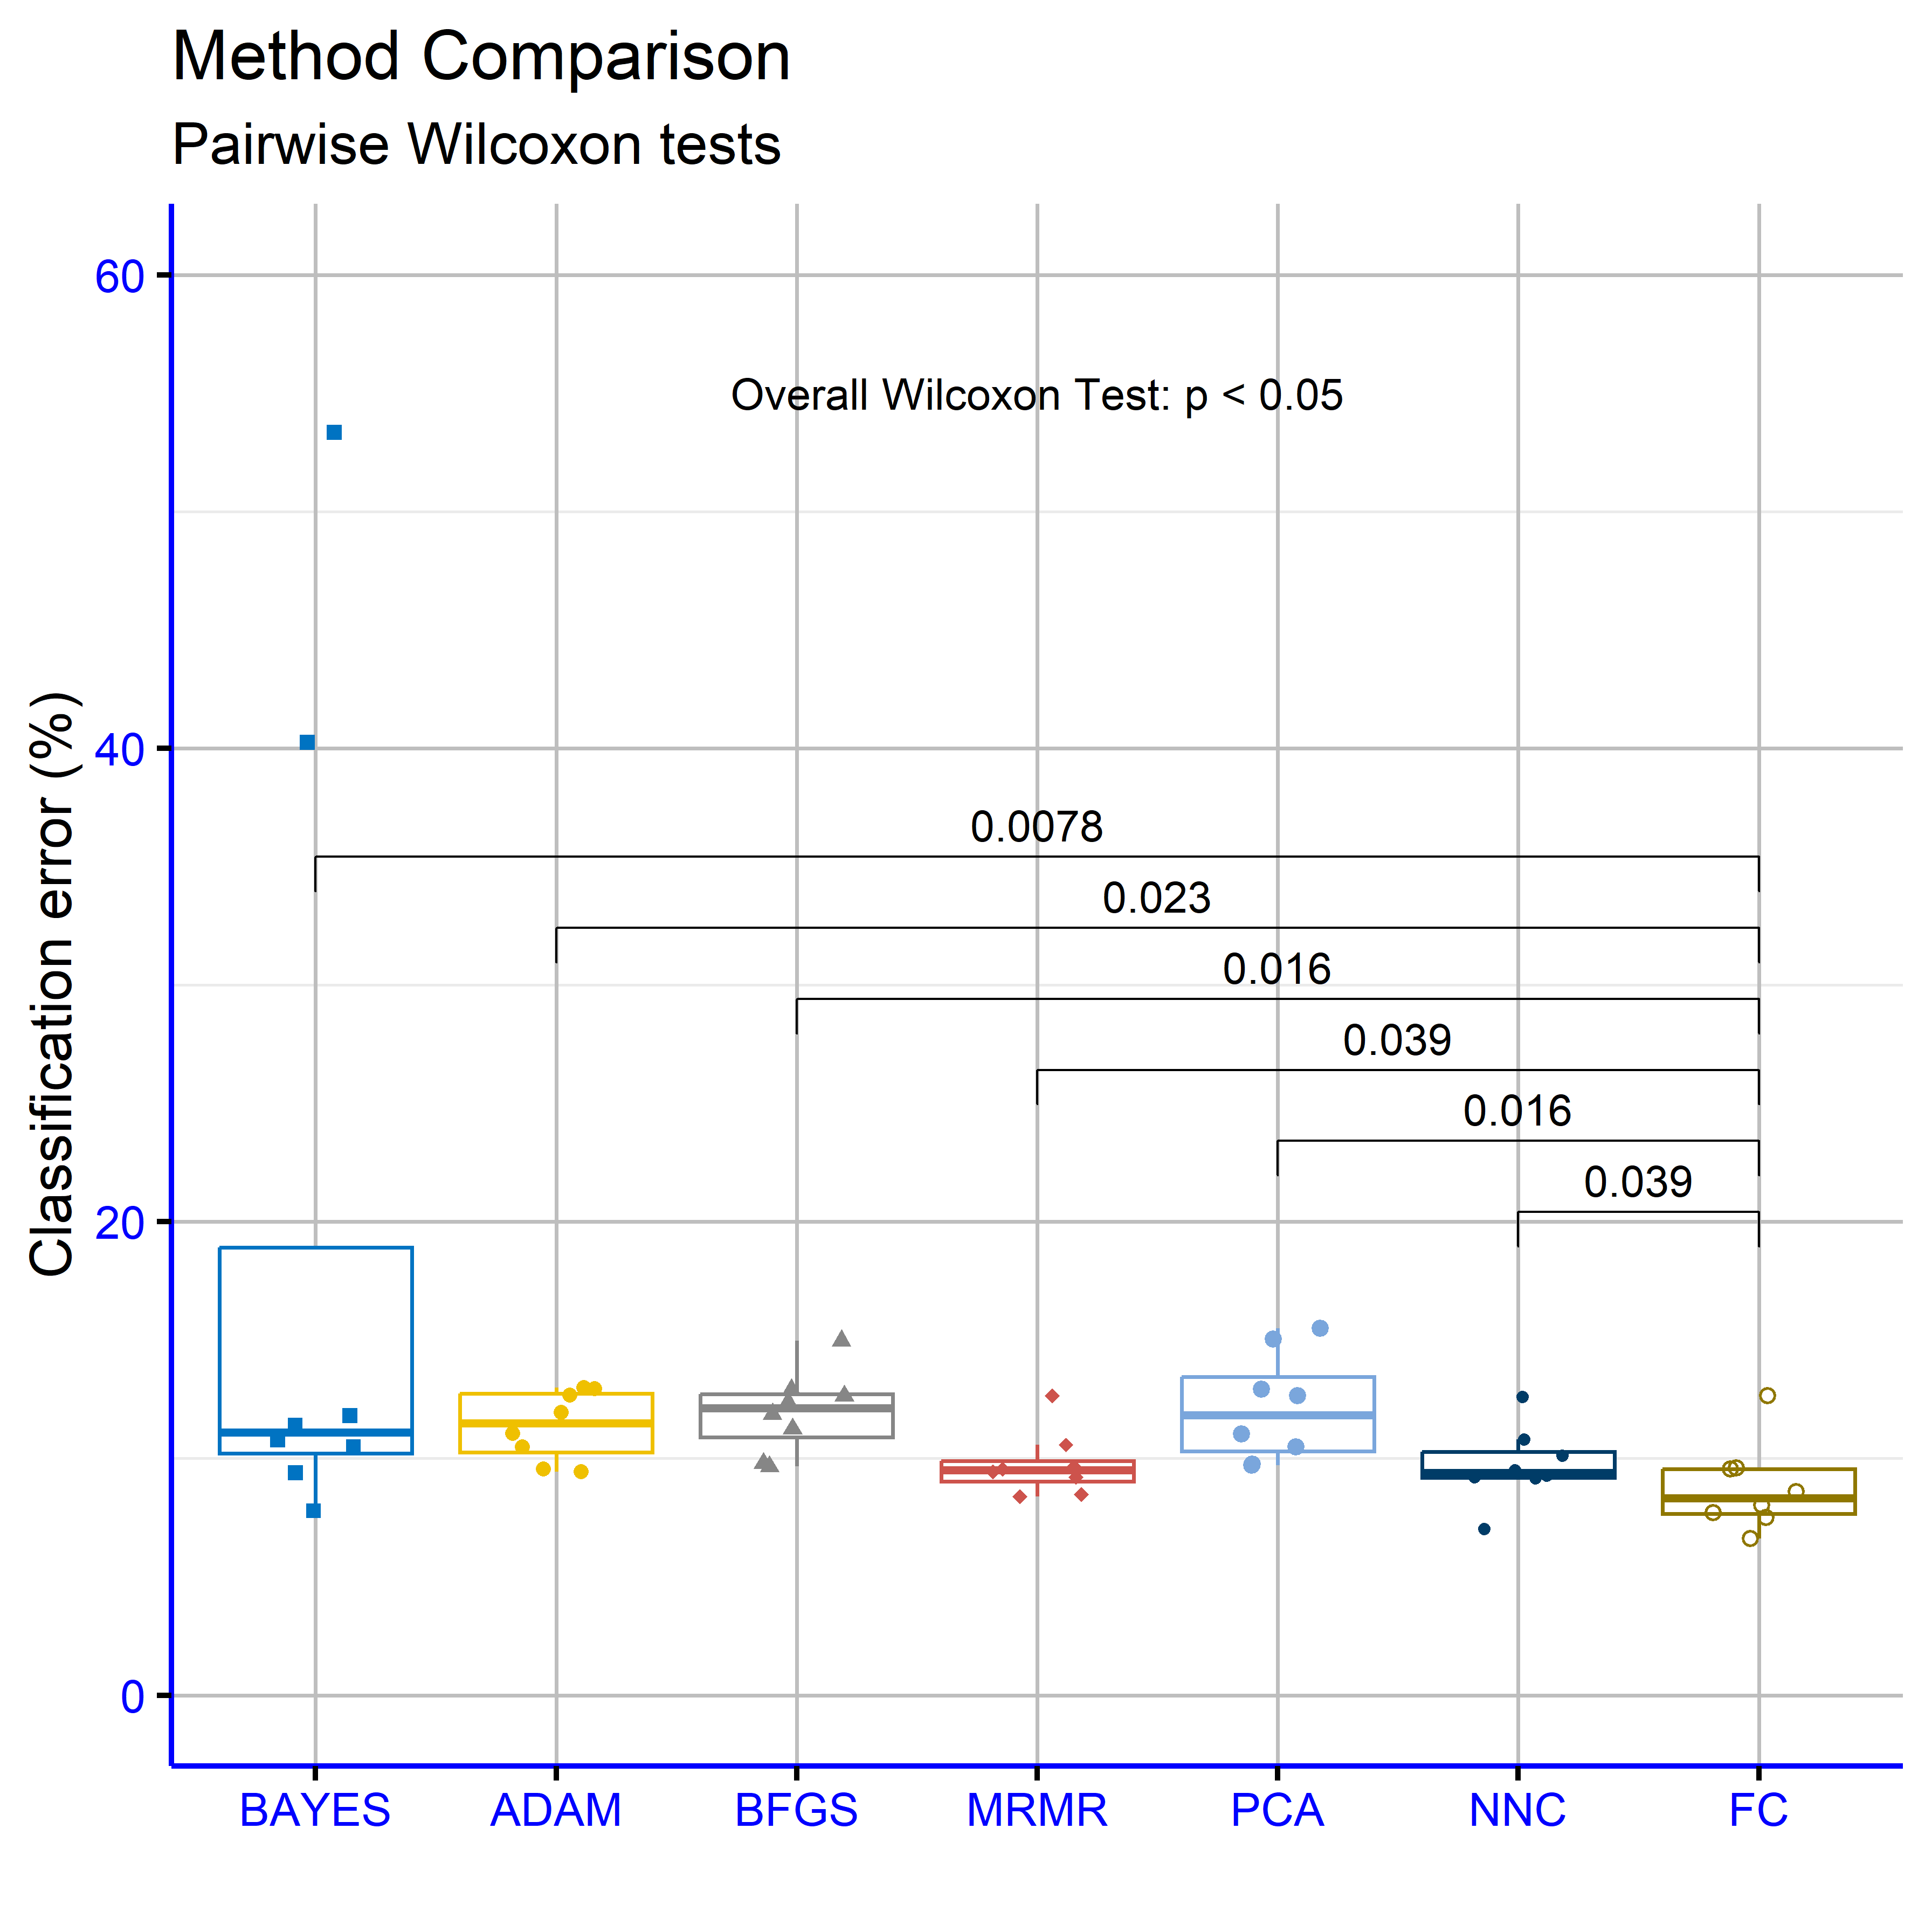
\includegraphics[scale=0.5]{statWilcoxon}

\caption{Statistical comparison of the used machine learning techniques.\label{fig:statExper}}
\end{figure}
The data in Table \ref{tab:experNF} present the classification error
rates for the \textquotedbl FC\textquotedbl{} machine learning model
across different numbers of constructed features ($N_{f}=1$, $N_{f}=2$,
and $N_{f}=3$) generated using Grammatical Evolution, spanning the
years 2014 to 2021. These results provide insights into the impact
of the number of features on the model's performance over time. For
$N_{f}=1$, the classification error rates exhibit variability across
the years, ranging from a minimum of 6.77\% in 2019 to a maximum of
12.68\% in 2017. The average error rate for this configuration is
9.03\%, indicating a relatively moderate level of accuracy overall.
The peak error in 2017 suggests possible challenges in that year's
data or specific interactions between the model and the constructed
feature set. For $N_{f}=2$, the classification error rates show a
slightly improved overall performance compared to $N_{f}=1$, with
an average error of 8.79\%. The error rates range from 6.62\% in 2019,
marking the lowest rate for this configuration, to 12.66\% in 2017,
the highest. These results indicate that adding one more feature generally
leads to improved accuracy, although the improvement is not uniform
across all years. For $N_{f}=3$, the classification error rates demonstrate
further improvement, with an average error of 8.63\%, which is the
lowest among the three configurations. The error rates range from
a minimum of 6.49\% in 2019 to a maximum of 12.46\% in 2017. The slightly
lower peak error compared to $N_{f}=1$ and $N_{f}=2$ suggests that
the inclusion of a third constructed feature enhances the model's
ability to capture data patterns more effectively. Across all configurations,
the year 2017 consistently exhibits the highest classification error
rates, irrespective of the number of features. This outlier suggests
specific data-related challenges or unique model behavior during that
year. Conversely, 2019 consistently shows the lowest error rates,
indicating favorable conditions for accurate classification during
that period. The trend in the average classification error rates decreasing
from 9.03\% for $N_{f}=1$ to 8.63\% for $N_{f}=3$ demonstrates that
the addition of constructed features through Grammatical Evolution
positively impacts the model's accuracy. However, the diminishing
returns between $N_{f}=2$ and $N_{f}=3$ suggest that the incremental
benefit of adding more features may plateau after a certain point.
In conclusion, the analysis reveals that increasing the number of
constructed features generally improves the accuracy of the \textquotedbl FC\textquotedbl{}
model. The results highlight the importance of balancing feature complexity
and model performance while considering the specific characteristics
of the data across different years.

\begin{table}[H]
\caption{Experiments with different number of constructed features for the
procedure that creates artificial features with Grammatical Evolution.\label{tab:experNF}}

\centering{}%
\begin{tabular}{|c|c|c|c|}
\hline 
YEAR & $N_{f}=1$ & $N_{f}=2$ & $N_{f}=3$\tabularnewline
\hline 
\hline 
2014 & 8.36\% & 8.04\% & 7.95\%\tabularnewline
\hline 
2015 & 8.10\% & 7.51\% & 7.24\%\tabularnewline
\hline 
2016 & 8.61\% & 8.60\% & 8.15\%\tabularnewline
\hline 
2017 & 12.68\% & 12.66\% & 12.46\%\tabularnewline
\hline 
2018 & 7.68\% & 7.72\% & 7.51\%\tabularnewline
\hline 
2019 & 6.77\% & 6.62\% & 6.49\%\tabularnewline
\hline 
2020 & 9.50\% & 9.61\% & 9.58\%\tabularnewline
\hline 
2021 & 10.53\% & 9.55\% & 9.62\%\tabularnewline
\hline 
\textbf{AVERAGE} & \textbf{9.03\%} & \textbf{8.79\%} & \textbf{8.63\%}\tabularnewline
\hline 
\end{tabular}
\end{table}
For Table \ref{tab:experNF}, a statistical analysis was conducted
using the Wilcoxon Test (Figure \ref{fig:statNf}) to compare classification
error rates among configurations with different numbers of constructed
features ($N_{f}=1,N_{f}=2$, and $N_{f}=3$). The results of the
test provide valuable insights into the statistical significance of
the differences in the performance of these configurations. The overall
result of the Wilcoxon Test, with p < 0.5, indicates that statistically
significant differences exist in at least one of the pairwise comparisons
between the configurations. Specifically, the comparison between $N_{f}=1$
and $N_{f}=2$ yields p = 0.15, which is not statistically significant.
This suggests that adding a second constructed feature does not lead
to a significant improvement in the model\textquoteright s performance.
On the other hand, the comparison between $N_{f}=1$ and $N_{f}=3$
shows p = 0.016, a statistically significant value. This indicates
that the inclusion of a third constructed feature substantially enhances
the model\textquoteright s accuracy compared to using only one feature.
The comparison between $N_{f}=2$ and $N_{f}=3$ also reveals a statistically
significant difference, with p = 0.023. This result suggests that
even the transition from $N_{f}=2$ to $N_{f}=3$ leads to an improvement
in performance, although the difference is less pronounced than between
$N_{f}=1$ and $N_{f}=3$. Overall, the analysis demonstrates that
increasing the number of constructed features from $N_{f}=1$ to $N_{f}=3$
results in a statistically significant improvement in the model\textquoteright s
accuracy. The comparison between $N_{f}=1$ and $N_{f}=2$ is not
statistically significant, possibly due to the limited impact of adding
only one additional feature. In contrast, the difference between $N_{f}=2$
and $N_{f}=3$ highlights that further increasing the number of features
continues to enhance performance, albeit to a lesser degree.
\begin{figure}[H]
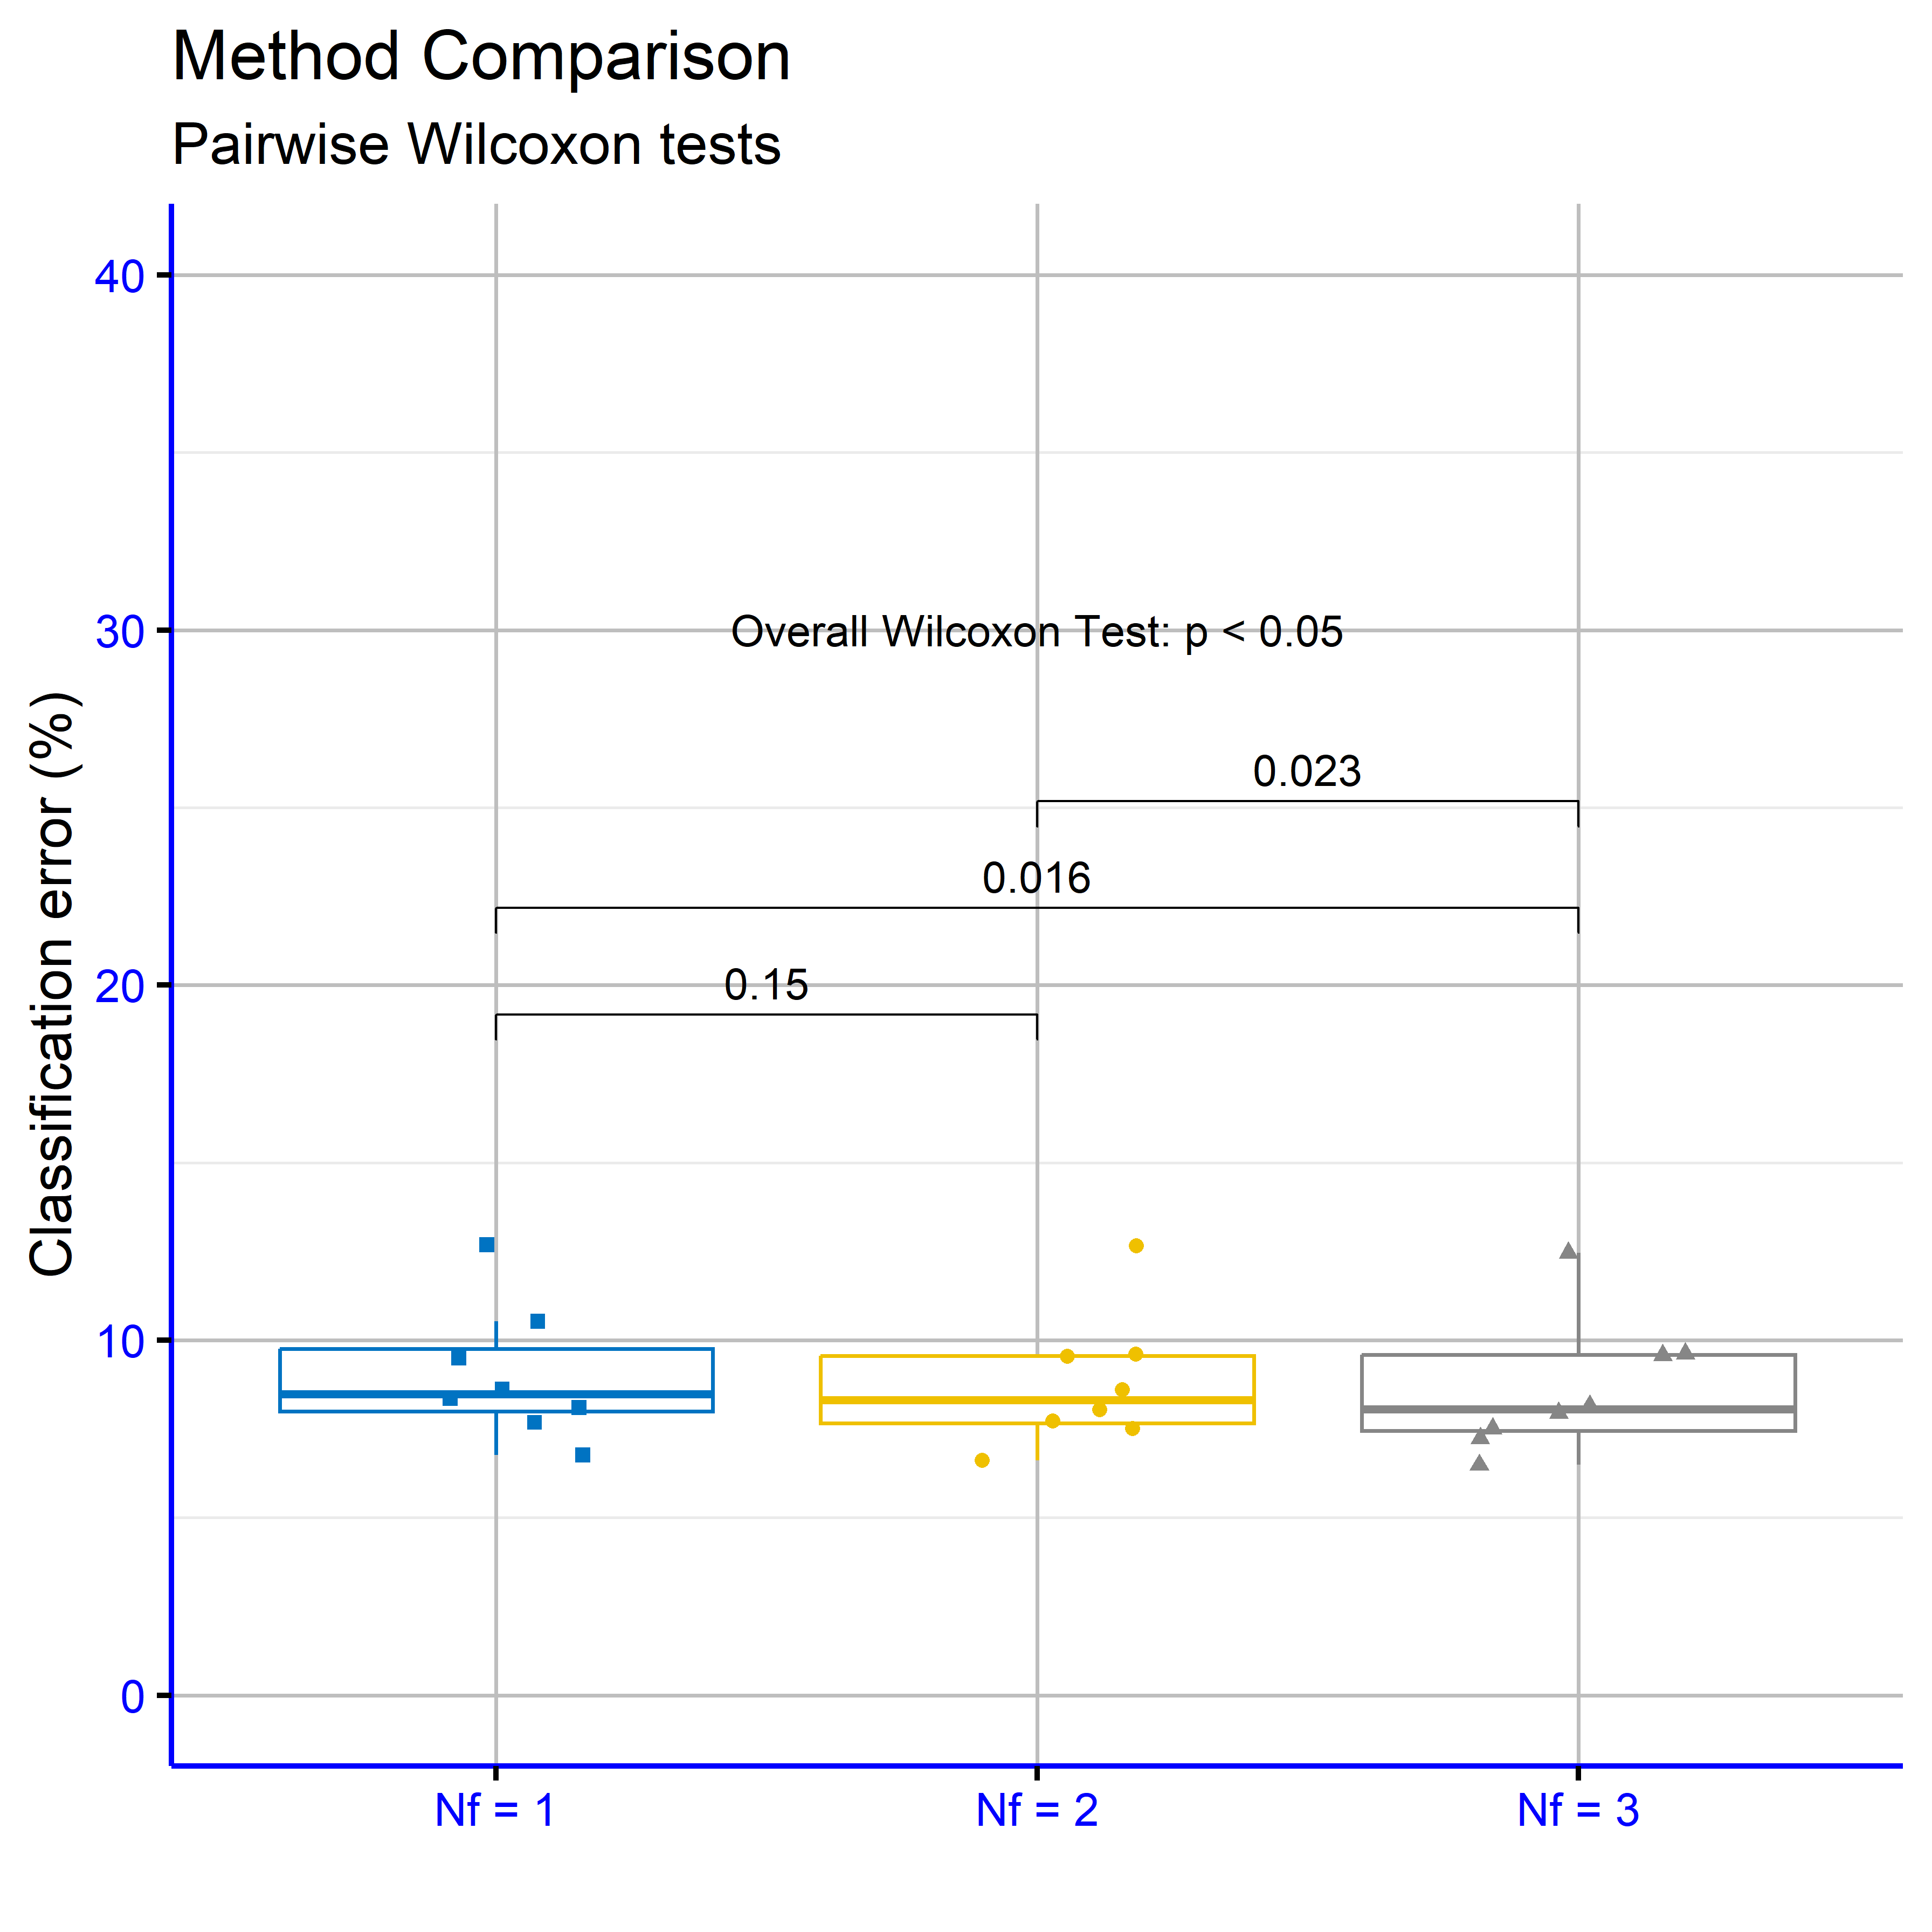
\includegraphics[scale=0.5]{statWilcoxon2}

\caption{Statistical comparison for the experiment involving different values
of the critical parameter $N_{f}$.\label{fig:statNf}}
\end{figure}


\section{Conclusions\label{sec:Conclusions}}

The study examines the application of feature construction techniques
for predicting the duration of forest fires using data collected in
Greece over a ten-year period. The methods utilized include Principal
Component Analysis (PCA), Minimum Redundancy Maximum Relevance (MRMR),
and Grammatical Evolution for constructing artificial features and
generating neural networks. The analysis focused on meteorological
parameters such as temperature, humidity, wind, and rainfall, which
significantly influence the behavior of forest fires. The research
concluded that the feature construction technique, using grammatical
evolution, outperforms other methods in terms of stability and accuracy.
The results indicated that this technique achieved the lowest error
rate in predicting fire duration compared to other approaches such
as PCA, MRMR, and traditional algorithms like Bayes and Adam. While
PCA proved effective for dimensionality reduction, it often led to
a loss of critical information. MRMR, though capable of identifying
relevant features, did not exhibit consistent performance across all
datasets. Traditional algorithms like Bayes showed significant variability,
with their performance heavily influenced by the data characteristics.
Statistical analysis using the Wilcoxon test demonstrated the clear
superiority of feature construction over other methods. This advantage
can be attributed to the technique's ability to adapt to the peculiarities
of the data, avoiding the information loss observed with other approaches.
Specifically, the method excelled in both accuracy and robustness.
The study's findings underscore the potential of advanced machine
learning techniques in addressing critical environmental challenges
such as forest fires. Future research could focus on integrating data
from diverse geographical regions or climatic conditions, developing
automated real-time monitoring systems, and combining advanced algorithms
for even more efficient analysis. Incorporating social and environmental
factors into predictive models could also offer a multidimensional
understanding of the causes and spread of fires. Overall, this study
highlights the importance of scientific approaches and technology
in tackling contemporary challenges posed by climate change and natural
disasters.

\section*{Declarations}
\begin{itemize}
\item Funding: Not Applicable.
\item Conflict of interest: The authors declare no conflicts of interest.
\item Ethics approval and consent to participate: Not Applicable.
\item Consent for publication: Not Applicable.
\item Data availability: The data used here are freely available from \url{https://www.fireservice.gr/en_US/synola-dedomenon}.
\item Materials availability: Not Applicable.
\item Code availability: The used code is freely available from \url{https://github.com/itsoulos/GlobalOptimus.git}
\item Author contribution: C.K., V.C.,A.M. and I.G.T. conceived of the idea
and the methodology, and C.K. and V.C. implemented the corresponding
software. C.K. and A.M. conducted the experiments, employing objective
functions as test cases, and provided the comparative experiments.
V.C. performed the necessary statistical tests. All authors have read
and agreed to the published version of the manuscript.
\end{itemize}
\begin{thebibliography}{10}
\bibitem{fire1}Gowlett, J.A.J. The discovery of fire by humans: a
long and convoluted process. Philosophical Transaction B, Biological
Sciences, volume 371, Issue 1696. June 5, 2016.

\bibitem{fire2}Heinonen, Keri. The Fire of Prometheus: More Than
Just a Gift to Humanity. Greek Mythology. November 19, 2024. Available
from: https://greek.mythologyworldwide.com/the-fire-of-prometheus-more-than-just-a-gift-to-humanity/
(accessed on November 29, 2024).

\bibitem{fire3}McCaffrey, S. (2004). Thinking of wildfire as a natural
hazard. Society and Natural Resources, 17(6), 509-516.

\bibitem{fire4}Patrick, Van Hees. The burning challenge of fire safety.
ISO, International Organization for Standardization. Available from:
https://www.iso.org/news/2014/11/Ref1906.html (accessed on December
3, 2024).

\bibitem{fire5}UNEP. United Nations Environment Programme. Number
of wildfires to rise by 50 per cent by 2100 and governments are not
prepared, experts warn. 23 February 2022. Available from: https://www.unep.org/news-and-stories/press-release/number-wildfires-rise-50-cent-2100-and-governments-are-not-prepared
(accessed on December 4, 2024).

\bibitem{fire_nasa}NASA. Carbon Dioxide, Vital Signs. October 2024.
Available from: https://climate.nasa.gov/vital-signs/carbon-dioxide/?intent=121
(accessed on November 29, 2024). 

\bibitem{fire_iliopoulos}Iliopoulos, N., Aliferis, I., \& Chalaris,
M. (2024). Effect of Climate Evolution on the Dynamics of the Wildfires
in Greece. Fire, 7(5), 162.

\bibitem{fire_giorgi}Giorgi, F. (2006). Climate change hot-spots.
Geophysical research letters, 33(8).

\bibitem{ai_climate}Satish, M., Prakash., Babu, S.M., Kumar, P.P.,
Devi, S., Reddy, K.P. Artificial Intelligence (AI) and the Prediction
of Climate Change Impacts. 2023. IEEE 5th International Conference
on Cybernetics, Cognition and Machine Learning Applications (ICCCMLA).

\bibitem{ai_ml}Walsh, Dylan. Tackling climate change with machine
learning. MIT Management Sloan School. Climate Change. October 24,
2023. Available from: https://mitsloan.mit.edu/ideas-made-to-matter/tackling-climate-change-machine-learning
(accessed on November 29, 2024). 

\bibitem{iso_ml}ISO. Machine Learning (ML): All there is to know.
International Organization for Standardization. Available from: https://www.iso.org/artificial-intelligence/machine-learning
(accessed on November 30, 2024).

\bibitem{ml_turing}Watson, Ian. (2012). How Alan Turing Invented
the Computer Age. Scientific American. Published: 26/04/2012.Available
from: https://blogs.scientificamerican.com/guest-blog/how-alan-turing-invented-the-computer-age/
(accessed on November 30, 2024). 

\bibitem{ml_review}Jain, P., Coogan, S. C., Subramanian, S. G., Crowley,
M., Taylor, S., \& Flannigan, M. D. (2020). A review of machine learning
applications in wildfire science and management. Environmental Reviews,
28(4), 478-505.

\bibitem{fire_manage}Xiao, H. (2023). Estimating fire duration using
regression methods. arXiv preprint arXiv:2308.08936.

\bibitem{fire_manage2}Linardos, V., Drakaki, M., Tzionas, P., \&
Karnavas, Y. L. (2022). Machine learning in disaster management: recent
developments in methods and applications. Machine Learning and Knowledge
Extraction, 4(2).

\bibitem{fire_bayes1}Sevinc, V., Kucuk, O., \& Goltas, M. (2020).
A Bayesian network model for prediction and analysis of possible forest
fire causes. Forest Ecology and Management, 457, 117723.

\bibitem{fire_bayes2}Chen, F., Jia, H., Du, E., Chen, Y., \& Wang,
L. (2024). Modeling of the cascading impacts of drought and forest
fire based on a Bayesian network. International Journal of Disaster
Risk Reduction, 111, 104716.

\bibitem{fire_bayes3}Kim, B., \& Lee, J. (2021). A Bayesian network-based
information fusion combined with DNNs for robust video fire detection.
Applied Sciences, 11(16), 7624.

\bibitem{fire_naive1}Nugroho, A. A., Iwan, I., Azizah, K. I. N.,
\& Raswa, F. H. (2019). Peatland Forest Fire Prevention Using Wireless
Sensor Network Based on Na�ve Bayes Classifier. KnE Social Sciences,
20-34.

\bibitem{fire_naive2}Zainul, M., \& Minggu, E. (2022). Classification
of Hotspots Causing Forest and Land Fires Using the Naive Bayes Algorithm.
Interdisciplinary Social Studies, 1(5), 555-567.

\bibitem{fire_naive3}Karo, I. M. K., Amalia, S. N., \& Septiana,
D. Wildfires Classification Using Feature Selection with K-NN, Na�ve
Bayes, and ID3 Algorithms. Journal of Software Engineering, Information
and Communication Technology (SEICT), 3(1), 15-24.

\bibitem{fire_log1}Vilar del Hoyo, L., Mart�n Isabel, M. P., \& Mart�nez
Vega, F. J. (2011). Logistic regression models for human-caused wildfire
risk estimation: analysing the effect of the spatial accuracy in fire
occurrence data. European Journal of Forest Research, 130, 983-996.

\bibitem{fire_log2}de Bem, P. P., de Carvalho J�nior, O. A., Matricardi,
E. A. T., Guimar�es, R. F., \& Gomes, R. A. T. (2018). Predicting
wildfire vulnerability using logistic regression and artificial neural
networks: a case study in Brazil\textquoteright s Federal District.
International journal of wildland fire, 28(1), 35-45.

\bibitem{fire_log3}Nhongo, E. J. S., Fontana, D. C., Guasselli, L.
A., \& Bremm, C. (2019). Probabilistic modelling of wildfire occurrence
based on logistic regression, Niassa Reserve, Mozambique. Geomatics,
Natural Hazards and Risk, 10(1), 1772-1792.

\bibitem{fire_log4}Peng, W., Wei, Y., Chen, G., Lu, G., Ye, Q., Ding,
R. \& Cheng, Z. (2023). Analysis of Wildfire Danger Level Using Logistic
Regression Model in Sichuan Province, China. Forests, 14(12), 2352.

\bibitem{fire_ann1}Hossain, F. A., Zhang, Y., Yuan, C., \& Su, C.
Y. (2019, July). Wildfire flame and smoke detection using static image
features and artificial neural network. In 2019 1st international
conference on industrial artificial intelligence (iai) (pp. 1-6).
IEEE.

\bibitem{fire_ann2}Lall, S., \& Mathibela, B. (2016, December). The
application of artificial neural networks for wildfire risk prediction.
In 2016 International Conference on Robotics and Automation for Humanitarian
Applications (RAHA) (pp. 1-6). IEEE.

\bibitem{fire_ann3}Sayad, Y. O., Mousannif, H., \& Al Moatassime,
H. (2019). Predictive modeling of wildfires: A new dataset and machine
learning approach. Fire safety journal, 104, 130-146.

\bibitem{fire_ann4}Gao, K., Feng, Z., \& Wang, S. (2022). Using multilayer
perceptron to predict forest fires in jiangxi province, southeast
china. Discrete Dynamics in Nature and Society, 2022(1), 6930812.

\bibitem{fire_rf1}Latifah, A. L., Shabrina, A., Wahyuni, I. N., \&
Sadikin, R. (2019, October). Evaluation of Random Forest model for
forest fire prediction based on climatology over Borneo. In 2019 International
Conference on Computer, Control, Informatics and its Applications
(IC3INA) (pp. 4-8). IEEE.

\bibitem{fire_rf2}Malik, A., Rao, M. R., Puppala, N., Koouri, P.,
Thota, V. A. K., Liu, Q., ... \& Gao, J. (2021). Data-driven wildfire
risk prediction in northern California. Atmosphere, 12(1), 109.

\bibitem{fire_rf3}Gao, C., Lin, H., \& Hu, H. (2023). Forest-fire-risk
prediction based on random forest and backpropagation neural network
of Heihe area in Heilongjiang province, China. Forests, 14(2), 170.

\bibitem{duration_andela}Andela, N., Morton, D. C., Giglio, L., Paugam,
R., Chen, Y., Hantson, S. \& Randerson, J. T. (2019). The Global Fire
Atlas of individual fire size, duration, speed and direction. Earth
System Science Data, 11(2), 529-552.

\bibitem{duration_surrogate}Kc, U., Aryal, J., Hilton, J., \& Garg,
S. (2021). A surrogate model for rapidly assessing the size of a wildfire
over time. Fire, 4(2), 20.

\bibitem{duration_wang}Liang, H., Zhang, M., \& Wang, H. (2019).
A neural network model for wildfire scale prediction using meteorological
factors. IEEE Access, 7, 176746-176755.

\bibitem{duration_xi}Xi, D. D., Dean, C. B., \& Taylor, S. W. (2021).
Modeling the duration and size of wildfires using joint mixture models.
Environmetrics, 32(6), e2685.

\bibitem{duration_wfca}WFCA. Western Fire Chiefs Association. How
Long Do Wildfires Last? October 2022. Available from: https://wfca.com/wildfire-articles/how-long-do-wildfires-last/
(accessed on December 4, 2024). 

\bibitem{genfc1}M.G. Smith, L. Bull, Genetic Programming with a Genetic
Algorithm for Feature Construction and Selection, Genet Program Evolvable
Mach \textbf{6}, pp. 265--281, 2005.

\bibitem{pca1}A. Ma\'{c}kiewicz, W. Ratajczak, Principal components
analysis (PCA). Computers \& Geosciences \textbf{19}, pp. 303-342,
1993.

\bibitem{pca_cadima}J. Cadima, I.T. Jolliffe, Principal component
analysis: a review and recent developments, National Library of Medicine.
2016. Available online: https://pmc.ncbi.nlm.nih.gov/articles/PMC4792409/
(accessed on 16 November 2024). 

\bibitem{pca_i2}i2tutorials. What are the Pros and Cons of the PCA?
October 1st, 2019. Available online: https://www.i2tutorials.com/what-are-the-pros-and-cons-of-the-pca/
(accessed on 16 November 2024). 

\bibitem{pca_park}S.C. Park, Physical Meaning of Principal Component
Analysis for Lattice Systems with Translational Invariance. arXiv
preprint arXiv:2410.22682, 2024.

\bibitem{pca_sarma}O. Sarma, M.A. Rather, S. Shahnaz, R.S. Barwal,
Principal Component Analysis of Morphometric Traits in Kashmir Merino
Sheep. Journal of Advances in Biology \& Biotechnology \textbf{27},
pp. 362-69, 2024.

\bibitem{pca_parente}C. Gambardella, R. Parente, A. Ciambrone, M.
Casbarra, A Principal Components Analysis -- Based Method for the
Detection of Cannabis Plants Using Representation data by Remote Sensing,
Knowledge Extractions from data Using Machine Learning, volume 6 (10),
2021.

\bibitem{pca_electric}M. Slavkovic, D. Jevtic, Face Recognition Using
Eigenface Approach, Serbian Journal of Electrical Engineering \textbf{9},
pp. 121-130, 2012.

\bibitem{pca_stock}C.A. Hargreaves, C.K. Mani, The Selection of Winning
Stocks Using Principal Component Analysis, American Journal of Marketing
Research \textbf{1}, pp. 183 -- 188, 2015.

\bibitem{pca_kernel}Z. Xu, F. Guo, H. Ma, X. Liu, L. Gao, On Optimizing
Hyperspectral Inversion of Soil Copper Content by Kernel Principal
Component Analysis. Remote Sensing \textbf{16}, 2024.

\bibitem{pca_zhang}H. Zhang, R. Srinivasa, X. Yang, S. Ahrentzen,
E.S. Coker, A. Alwisy, Factors influencing indoor air pollution in
buildings using PCA -- LMBP neural network: A case study of a university
campus, Building and environment \textbf{225}, 2022.

\bibitem{lm_paper}M.I. Lourakis, A brief description of the Levenberg-Marquardt
algorithm implemented by levmar, Foundation of Research and Technology
\textbf{4}, pp. 1-6, 2005.

\bibitem{pca_svm}B.A. Akinnuwesi, B.O. Macaulay, B.S. Aribisala,
Breast cancer risk assessment and early diagnosis using Principal
Component Analysis and support vector machine techniques, Informatics
in medicine unlocked \textbf{21}, 100459, 2020.

\bibitem{svm}M. Awad, R. Khanna, M. Awad, R. Khanna, Support vector
machines for classification. Efficient learning machines: Theories,
concepts, and applications for engineers and system designers, pp.
39-66, 2015.

\bibitem{pca_guan}R. Guan, Predicting forest fire with linear regression
and random forest, Highlights in Science, Engineering and Technology
\textbf{44}, pp. 1-7, 2023.

\bibitem{pca_nikolov}N. Nikolov, P. Bothwell, J. Snook, Developing
a gridded model for probabilistic forecasting of wildland-fire ignitions
across the lower 48 States. USFS-CSU Joint Venture Agreement Phase
2 (2019-2021)-Final Report. Fort Collins, CO: US Department of Agriculture,
Forest Service, Rocky Mountain Research Station. 33p, 2022.

\bibitem{pca_nikolov2}N. Nikolov, P. Bothwell, J. Snook, Probalistic
forecasting of lightning strikes over the Continental USA and Alaska:
Model development and verification. Scientific Journal, Fire (7).
Available from: https://research.fs.usda.gov/treesearch/68447 (accessed
20 November 2024). 

\bibitem{mrmr1} C. Ding, H. Peng, Minimum redundancy feature selection
from microarray gene expression data. Journal of bioinformatics and
computational biology \textbf{3}, pp. 185-205, 2005.

\bibitem{mrmr2}S. Ramirez -- Gallego, I. Lastra, D. Martinez --
Rego, V. Bolon -- Canedo, J.M. Benitez, F. Herrera, A. Alonso --
Betanzos, Fast-mRMR: Fast Minimum Redundancy Maximum Relevance Algorithm
for High -- Dimensional Big Data, International Journal of Intelligent
Systems \textbf{32}, pp. 134 -- 152, 2017.

\bibitem{mrmr_zhao}Zhao, Z., Anand, R., \& Wang, M. (2019, October).
Maximum relevance and minimum redundancy feature selection methods
for a marketing machine learning platform. In 2019 IEEE international
conference on data science and advanced analytics (DSAA) (pp. 442-452).
IEEE.

\bibitem{random_forest}S.J. Rigatti, Random forest. Journal of Insurance
Medicine \textbf{47}, pp. 31-39, 2017.

\bibitem{mrmr_wu}Wu, H., Yang, T., Li, H., \& Zhou, Z. (2023). Air
quality prediction model based on mRMR--RF feature selection and
ISSA--LSTM. Scientific Reports, 13(1), 12825.

\bibitem{mrmr_elbeltagi}Elbeltagi, A., Nagy, A., Szabo, A., Nxumalo,
G.S., Bodi, E.B., Tamas, J. Hyperspectral indices data fusion-based
machine learning enhanced by MRMR algorithm for estimating maize chlorophyll
content. Frontiers in Plant Science, Section Technical Advances in
Plant Science, volume 15, October 2024. 

\bibitem{mrmr_liu}Liu, J., Sun, H., Li, Y., Fang, W., \& Niu, S.
(2020). An improved power system transient stability prediction model
based on mRMR feature selection and WTA ensemble learning. Applied
Sciences, 10(7), 2255.

\bibitem{eml}Dietterich, T. G. (2000, June). Ensemble methods in
machine learning. In International workshop on multiple classifier
systems (pp. 1-15). Berlin, Heidelberg: Springer Berlin Heidelberg.

\bibitem{mrmr_eristi}Eristi, B. (2024). A New Approach based on Deep
Features of Convolutional Neural Networks for Partial Discharge Detection
in Power Systems. IEEE Access.

\bibitem{mrmr_zhang}Li, Y., Zhang, Y., Zhu, H., Yan, R., Liu, Y.,
Sun, L., \& Zeng, Z. (2015). Recognition algorithm of acoustic emission
signals based on conditional random field model in storage tank floor
inspection using inner detector. Shock and Vibration, 2015(1), 173470.

\bibitem{mrmr_razmi}Karamouz, M., Zahmatkesh, Z., Nazif, S., \& Razmi,
A. (2014). An evaluation of climate change impacts on extreme sea
level variability: Coastal area of New York City. Water resources
management, 28, 3697-3714.

\bibitem{ge1}M. O\textquoteright Neill, C. Ryan, Grammatical evolution,
IEEE Trans. Evol. Comput. \textbf{5,}pp. 349--358, 2001.

\bibitem{nnc}I.G. Tsoulos, D. Gavrilis, E. Glavas, Neural network
construction and training using grammatical evolution, Neurocomputing
\textbf{72}, pp. 269-277, 2008.

\bibitem{nnc_amide1}G.V. Papamokos, I.G. Tsoulos, I.N. Demetropoulos,
E. Glavas, Location of amide I mode of vibration in computed data
utilizing constructed neural networks, Expert Systems with Applications
\textbf{36}, pp. 12210-12213, 2009.

\bibitem{nnc_de}I.G. Tsoulos, D. Gavrilis, E. Glavas, Solving differential
equations with constructed neural networks, Neurocomputing \textbf{72},
pp. 2385-2391, 2009.

\bibitem{nnc_feas}I.G. Tsoulos, G. Mitsi, A. Stavrakoudis, S. Papapetropoulos,
Application of Machine Learning in a Parkinson's Disease Digital Biomarker
Dataset Using Neural Network Construction (NNC) Methodology Discriminates
Patient Motor Status, Frontiers in ICT 6, 10, 2019.

\bibitem{nnc_student}V. Christou, I.G. Tsoulos, V. Loupas, A.T. Tzallas,
C. Gogos, P.S. Karvelis, N. Antoniadis, E. Glavas, N. Giannakeas,
Performance and early drop prediction for higher education students
using machine learning, Expert Systems with Applications \textbf{225},
120079, 2023.

\bibitem{nnc_autism}E.I. Toki, J. Pange, G. Tatsis, K. Plachouras,
I.G. Tsoulos, Utilizing Constructed Neural Networks for Autism Screening,
Applied Sciences \textbf{14}, 3053, 2024.

\bibitem{bnf1}J. W. Backus. The Syntax and Semantics of the Proposed
International Algebraic Language of the Zurich ACM-GAMM Conference.
Proceedings of the International Conference on Information Processing,
UNESCO, 1959, pp.125-132.

\bibitem{fc1}Dimitris Gavrilis, Ioannis G. Tsoulos, Evangelos Dermatas,
Selecting and constructing features using grammatical evolution, Pattern
Recognition Letters \textbf{29},pp. 1358-1365, 2008. 

\bibitem{fc2}Dimitris Gavrilis, Ioannis G. Tsoulos, Evangelos Dermatas,
Neural Recognition and Genetic Features Selection for Robust Detection
of E-Mail Spam, Advances in Artificial Intelligence Volume 3955 of
the series Lecture Notes in Computer Science pp 498-501, 2006.

\bibitem{fc3}George Georgoulas, Dimitris Gavrilis, Ioannis G. Tsoulos,
Chrysostomos Stylios, Jo�o Bernardes, Peter P. Groumpos, Novel approach
for fetal heart rate classification introducing grammatical evolution,
Biomedical Signal Processing and Control \textbf{2},pp. 69-79, 2007 

\bibitem{fc4}Otis Smart, Ioannis G. Tsoulos, Dimitris Gavrilis, George
Georgoulas, Grammatical evolution for features of epileptic oscillations
in clinical intracranial electroencephalograms, Expert Systems with
Applications \textbf{38}, pp. 9991-9999, 2011 

\bibitem{fc5}A. T. Tzallas, I. Tsoulos, M. G. Tsipouras, N. Giannakeas,
I. Androulidakis and E. Zaitseva, Classification of EEG signals using
feature creation produced by grammatical evolution, In: 24th Telecommunications
Forum (TELFOR), pp. 1-4, 2016.

\bibitem{rbf1}J. Park and I. W. Sandberg, Universal Approximation
Using Radial-Basis-Function Networks, Neural Computation 3, pp. 246-257,
1991.

\bibitem{rbf2}H. Yu, T. Xie, S. Paszczynski, B. M. Wilamowski, Advantages
of Radial Basis Function Networks for Dynamic System Design, in IEEE
Transactions on Industrial Electronics \textbf{58}, pp. 5438-5450,
2011.

\bibitem{nn1}C. Bishop, Neural Networks for Pattern Recognition,
Oxford University Press, 1995.

\bibitem{nn2}G. Cybenko, Approximation by superpositions of a sigmoidal
function, Mathematics of Control Signals and Systems \textbf{2}, pp.
303-314, 1989.

\bibitem{powell}M.J.D Powell, A Tolerant Algorithm for Linearly Constrained
Optimization Calculations, Mathematical Programming \textbf{45}, pp.
547-566, 1989.

\bibitem{weka_main}M. Hall, F. Frank, G. Holmes, B. Pfahringer, P.
Reutemann, I.H. Witten, The WEKA data mining software: an update.
ACM SIGKDD explorations newsletter \textbf{11}, pp. 10-18, 2009.

\bibitem{weka_education1}S.B. Aher, L.M.R.J. Lobo, Data mining in
educational system using weka. In International conference on emerging
technology trends, Foundation of Computer Science \textbf{3}, pp.
20-25, 2011.

\bibitem{weka_education2}S. Hussain, N.A. Dahan, F.M. Ba-Alwib, N.
Ribata, Educational data mining and analysis of students\textquoteright{}
academic performance using WEKA. Indonesian Journal of Electrical
Engineering and Computer Science \textbf{9}, pp. 447-459, 2018.

\bibitem{weka_medical1}A.K. Sigurdardottir, H. Jonsdottir, R. Benediktsson,
Outcomes of educational interventions in type 2 diabetes: WEKA data-mining
analysis. Patient education and counseling \textbf{67}, pp. 21-31,
2007.

\bibitem{weka_medical2}M.N. Amin, A. Habib, Comparison of different
classification techniques using WEKA for hematological data. American
Journal of Engineering Research \textbf{4}, pp. 55-61, 2015.

\bibitem{naive_bayes}G.I. Webb, E. Keogh, R. Miikkulainen, Na�ve
Bayes, Encyclopedia of machine learning \textbf{15}, pp. 713-714,
2010.

\bibitem{nn_adam}D. P. Kingma, J. L. Ba, ADAM: a method for stochastic
optimization, in: Proceedings of the 3rd International Conference
on Learning Representations (ICLR 2015), pp. 1--15, 2015.

\bibitem{mlpack}Ryan R. Curtin, James R. Cline, N. P. Slagle, William
B. March, Parikshit Ram, Nishant A. Mehta, Alexander G. Gray, MLPACK:
A Scalable C++ Machine Learning Library, Journal of Machine Learning
Research \textbf{14}, pp. 801-805, 2013.

\bibitem{nnc_softx}I.G. Tsoulos, A. Tzallas, D. Tsalikakis, NNC:
A tool based on Grammatical Evolution for data classification and
differential equation solving, SoftwareX \textbf{10}, 100297, 2019.

\bibitem{qfc}I.G. Tsoulos, QFC: A Parallel Software Tool for Feature
Construction, Based on Grammatical Evolution. Algorithms \textbf{15},
295, 2022.

\end{thebibliography}

\end{document}
